\documentclass[aspectratio=169,11pt]{beamer}
\usepackage{beamertemplate}
\usepackage{graphicx}
\usepackage{url}
\usepackage{textcomp}
\usepackage{eurosym}
\usepackage[normalem]{ulem}
\usepackage{ragged2e}
\usepackage{etoolbox}
\apptocmd{\itemize}{\justifying}{}{}
\AtBeginEnvironment{frame}{\justifying}

% Las secciones no actuales se muestran atenuadas al 30 %
\setbeamertemplate{section in toc shaded}[default][30]

% Repite el índice al empezar cada sección, resaltando la que comienza
\AtBeginSection[]{%
  \begin{frame}{Índice}
  \small
  \tableofcontents[currentsection]
  \end{frame}
}

\title[SSI -- Tema 1.2]{Introducción a la Seguridad Informática y de la Información}
\subtitle{Seguridad en Sistemas Informáticos --- Tema 1.2}
\author{José Luis Martínez}
\institute{Universidad de Castilla-La Mancha}
\date{Curso 2026/27}

\begin{document}

\begin{frame}[plain]\titlepage\end{frame}

\begin{frame}{Índice}
\small
\tableofcontents
\end{frame}

\section{Introducción: la información, los incidentes y las amenazas}

\begin{frame}{Introducción}
\small
\begin{columns}[c]
\begin{column}{0.52\textwidth}
  \begin{itemize}
  \item La información es valor, y ese valor se puede usar para múltiples fines
    \begin{itemize}
    \item Ver \href{https://www.youtube.com/watch?v=NPE7i8wuupk&feature=youtu.be}{vídeo}
    \item Concepto de privacidad
    \end{itemize}
  \item \href{https://www.incibe.es/protege-tu-empresa/blog/historias-reales-me-han-cifrado-disco-duro}{Incidentes}
  \item \href{https://www.eldiario.es/hojaderouter/seguridad/mikko-hypponnen-ciberguerra-ciberarmas-internet_1_3551002.html}{Ciberguerras}
  \end{itemize}
\end{column}
\begin{column}{0.46\textwidth}
\begin{center}
\includegraphics[width=\textwidth,height=0.72\textheight,keepaspectratio]{img/sl004.jpg}
\end{center}
\end{column}
\end{columns}
\end{frame}

\begin{frame}[allowframebreaks]{Introducción}
\small
  \begin{itemize}
  \item Ver \href{https://www.youtube.com/watch?v=7UPe_fxOz8M}{video}
  \item ¿Esto ocurre realmente?
  \item Ataques en tiempo real  
  \begin{itemize}
      \item \href{http://www.digitalattackmap.com/\#anim=1&color=0&country=ALL&time=16251&view=ma}{Digital Attack Map}
      \item \href{http://globalsecuritymap.com/}{Global Security Map}
      \item \href{http://www.akamai.com/html/technology/dataviz1.html}{Real Time Web Monitor}
      \item \href{https://ics-radar.shodan.io/}{Shodan Radar}
      \item \href{http://www.tecnoxplora.com/internet/googlerecrea-atlas-mundial-ataquesddos_2013102700161.html}{Google}
      \item \href{https://cybermap.kaspersky.com/es}{Kaspersky}
      \item \href{https://www.fireeye.com/cyber-map/threat-map.html}{Fireeye}
      \item \href{https://threatmap.checkpoint.com/}{Checkpoint}
    \end{itemize}
  \end{itemize}
\end{frame}

\begin{frame}{Introducción}
\small
\begin{columns}[c]
\begin{column}{0.52\textwidth}
  \begin{itemize}
  \item \href{https://www.incibe.es/protege-tu-empresa/blog/ataques-reputacion-marcas-personales-corporativas}{Ataques a la reputación de marcas personales y corporativas (INCIBE)}
  \item \href{https://www.eleconomista.es/tecnologia/amp/8493660/El-CEO-de-Securitas-declarado-en-banca-rota-despues-de-que-le-hayan-hackeado-su-identidad-online}{El CEO de Securitas, en bancarrota tras el robo de su identidad online (El Economista)}
  \item Cada día hay brechas de seguridad que afectan a empresas importantes
    \begin{itemize}
    \item Vector de ataque: Ingeniería Social (spear phising + data leaks + ransomware + \dots{})
    \end{itemize}
  \end{itemize}
\end{column}
\begin{column}{0.46\textwidth}
\begin{center}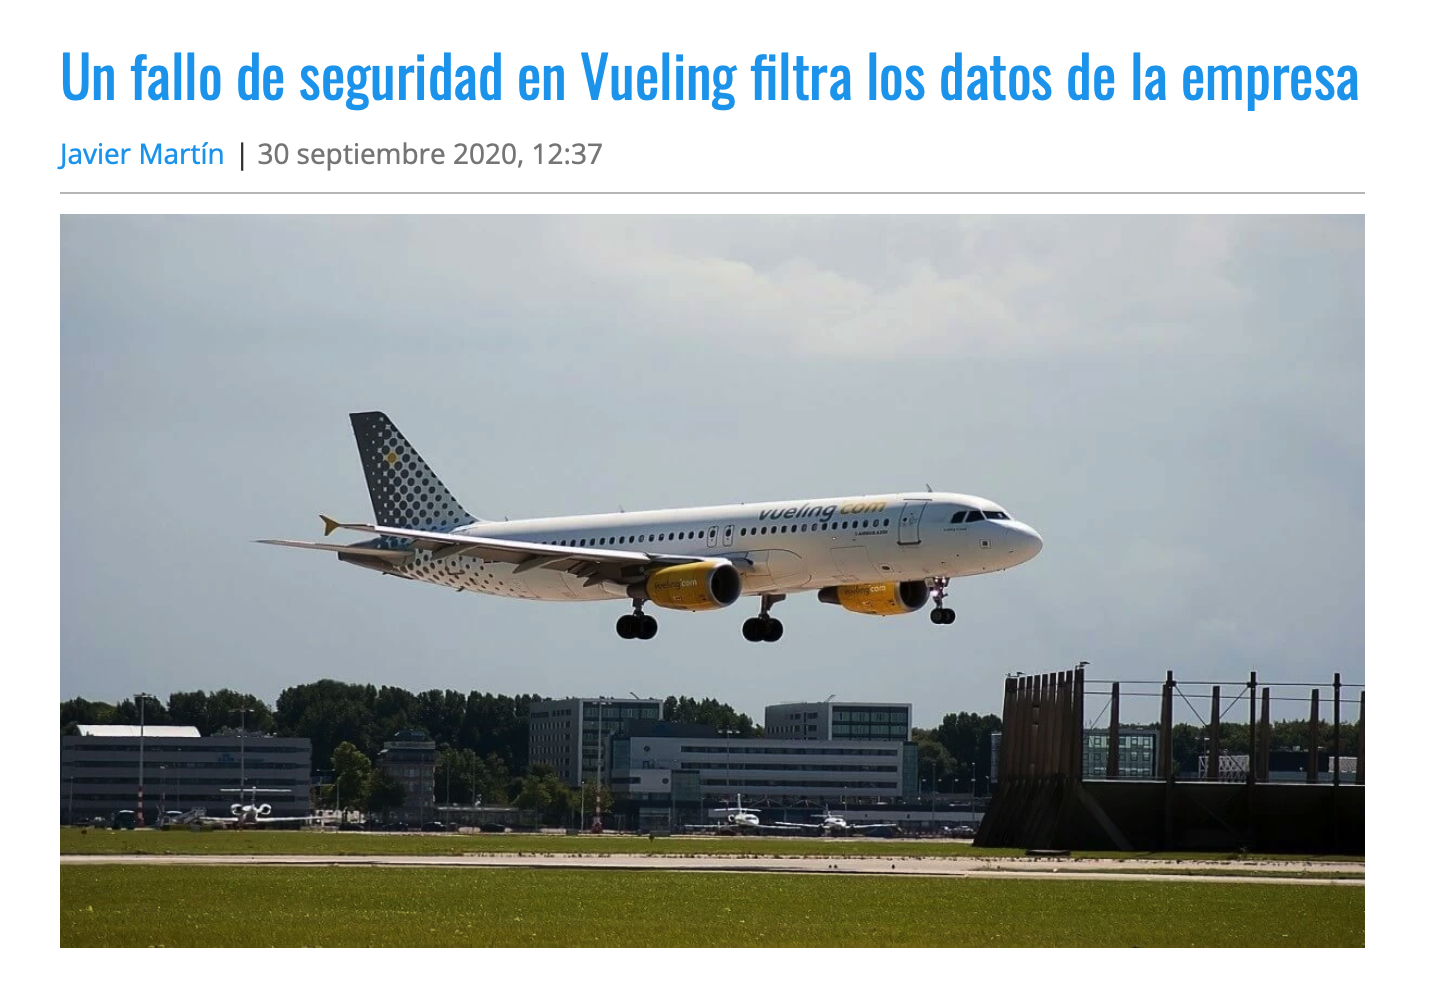
\includegraphics[width=\textwidth,height=0.72\textheight,keepaspectratio]{img/sl006.png}
\end{center}
\end{column}
\end{columns}
\end{frame}

\begin{frame}{Introducción}
\footnotesize
\begin{columns}[c]
\begin{column}{0.56\textwidth}
  \begin{itemize}
  \item principales deficiencias que explotan:
    \begin{itemize}
    \item Contraseñas débiles o comprometidas o filtradas
    \item Software no seguro
    \item Dirigir tráfico por canales inseguros
    \item Confiar en sitios web inseguros
    \end{itemize}
  \item qué quieres:
    \begin{itemize}
    \item Archivos de clientes
    \item Datos de gestión / Registros financieros

    \item Mensajes de correo electrónico
    \item Contraseñas
    \end{itemize}
  \item ¿Para qué?
    \begin{itemize}
    \item Extorsión
    \item Espionaje: comercial o político
    \item Venta en darkweb
    \end{itemize}
  \end{itemize}
\end{column}
\begin{column}{0.42\textwidth}
\begin{center}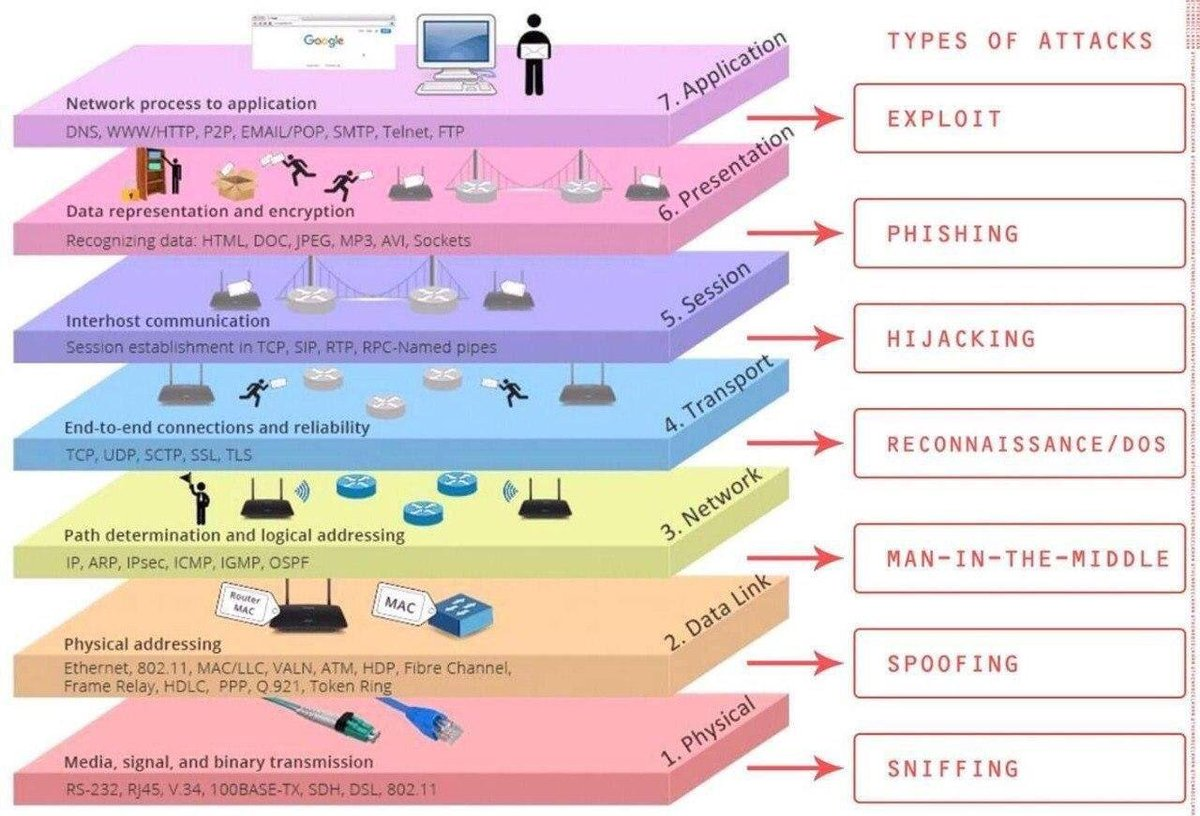
\includegraphics[width=\textwidth,height=0.78\textheight,keepaspectratio]{img/sl007.jpg}
\end{center}
\end{column}
\end{columns}
\end{frame}

\begin{frame}[allowframebreaks]{Introducción}
\small
  Más amenazas cada año:  
\begin{itemize}
  \item Los avisos de vulnerabilidades no dejan de crecer, tanto en TI como en sistemas industriales (ICS-CERT).
  \item El ransomware se ha profesionalizado y golpea a todos los sectores; en industria, la fabricación es de los más atacados.
  \item Un incidente ya no es solo "perder datos": puede parar servicios esenciales (agua, energía, salud, producción).
  \item Fuente: ICS-CERT / icsadvisoryproject.com
  \end{itemize}
\end{frame}

\begin{frame}[plain]
\centering
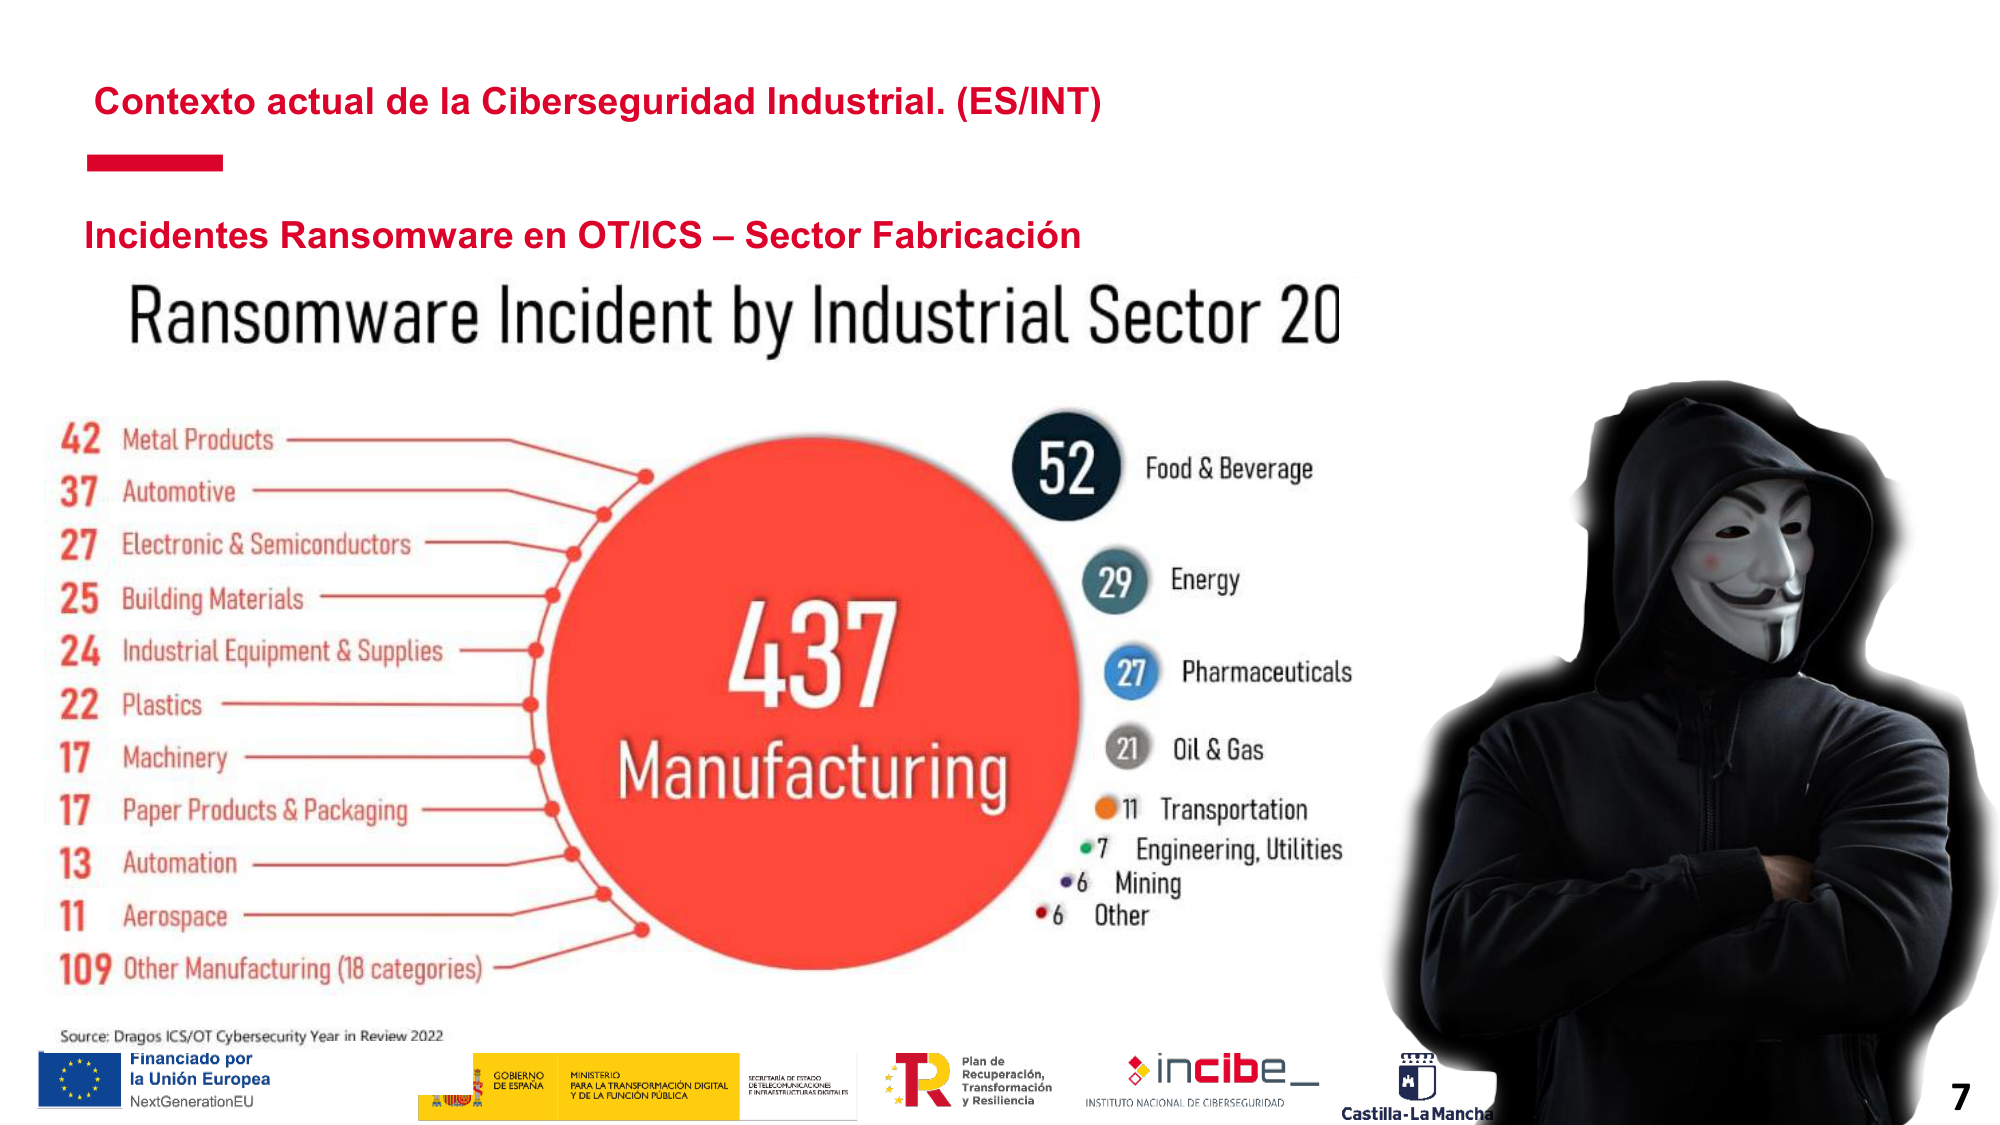
\includegraphics[trim=0 72 0 0,clip,width=\paperwidth,height=\paperheight,keepaspectratio]{img/sl008.png}
\end{frame}

\begin{frame}[allowframebreaks]{Introducción}
\small
  \begin{itemize}
  \item Geopolítica y objetivos críticos
  \item La ciberguerra acompaña a los conflictos: infraestructuras críticas y empresas son objetivo.
  \item Caso real: American Water (mayor operadora de agua de EE. UU., 14 M de personas) sufrió una brecha que la obligó a suspender la facturación.
  \item La economía del ransomware
  \item Tras el cifrado llega la extorsión: los grupos publican lo robado en webs de leaks (TOR). Rastreable en ransomware.live.
  \item Fuente: ransomware.live
  \end{itemize}
\end{frame}

\begin{frame}[plain]
\centering
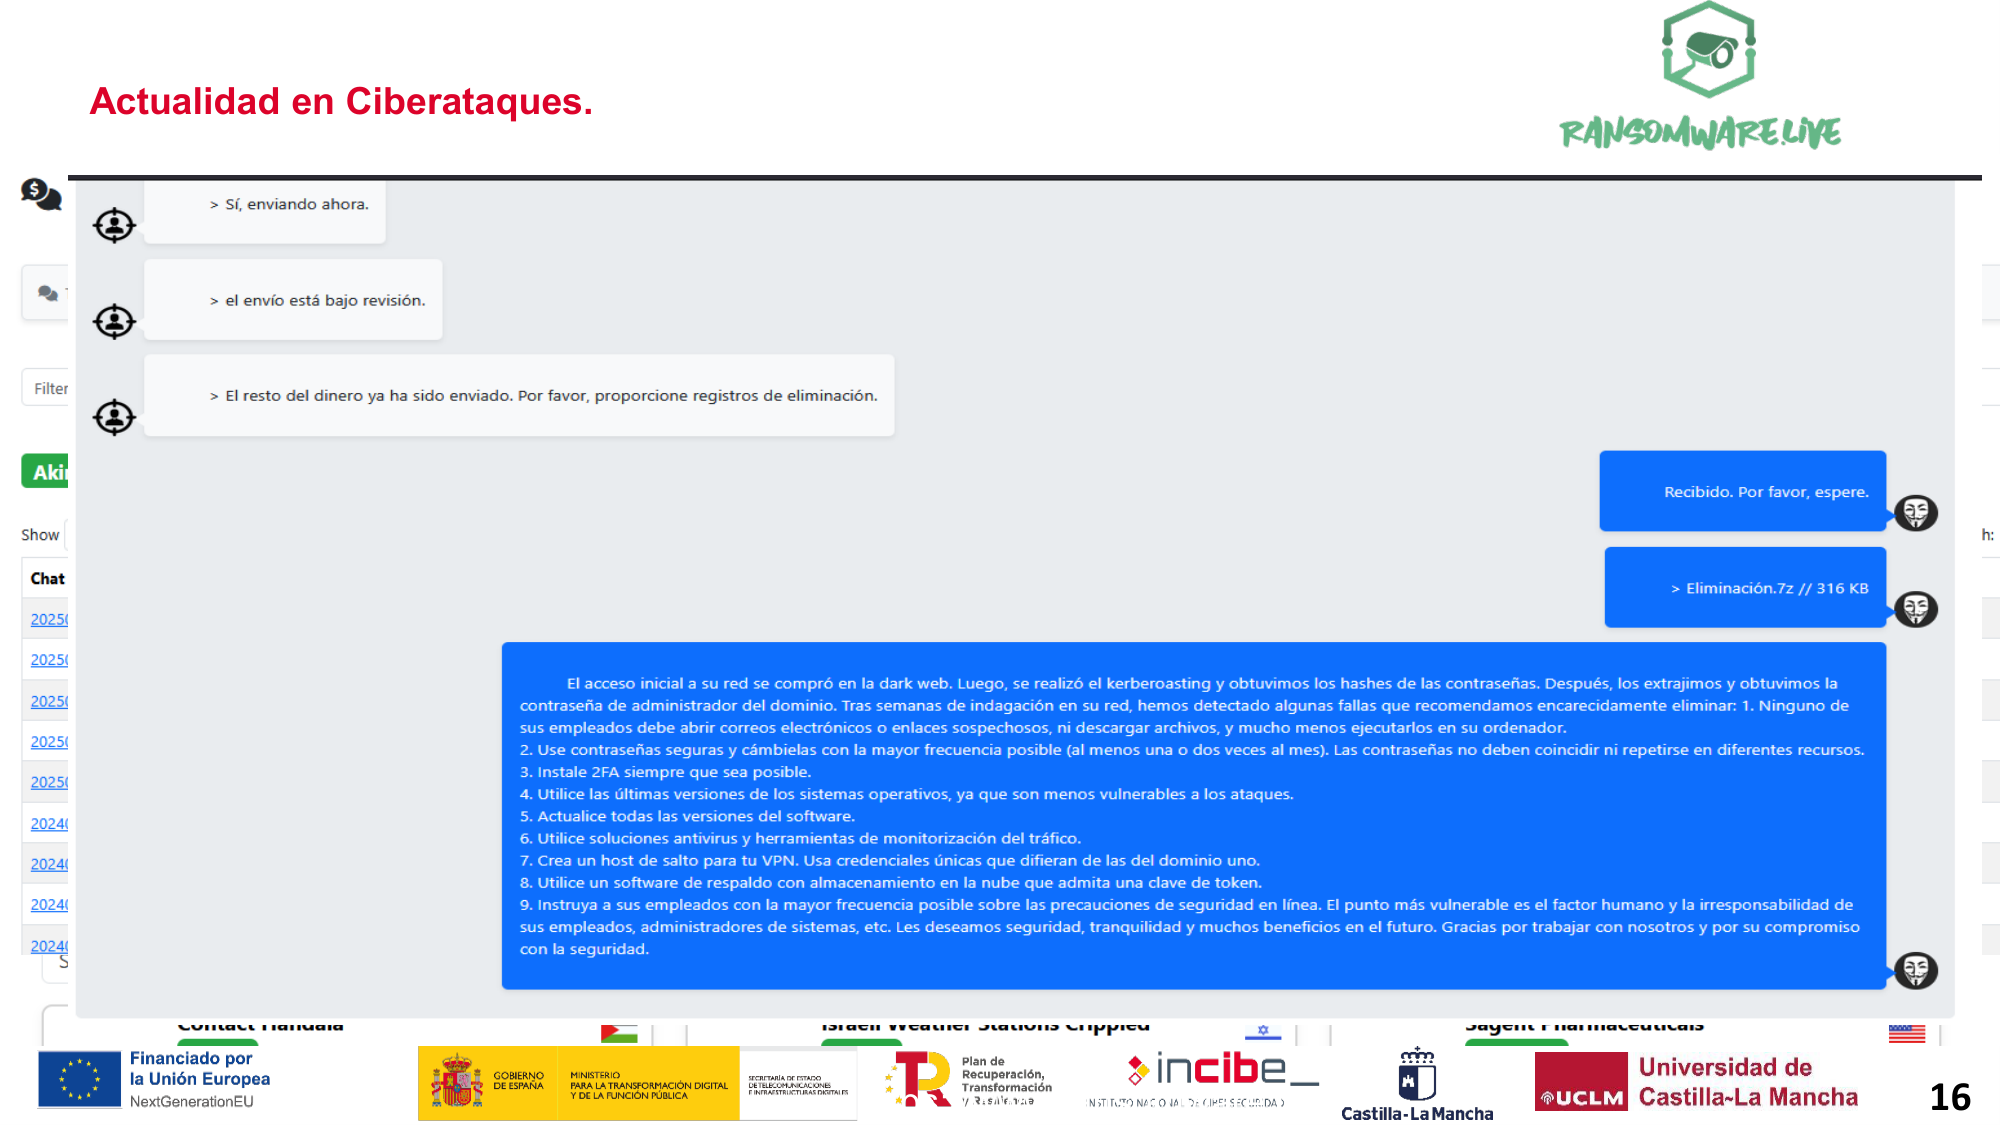
\includegraphics[trim=0 72 0 0,clip,width=\paperwidth,height=\paperheight,keepaspectratio]{img/sl009.png}
\end{frame}

\begin{frame}[allowframebreaks]{Introducción}
\small
  \begin{itemize}
  \item Exposición innecesaria en Internet
  \item Buscadores como Shodan.io localizan dispositivos y servicios accesibles desde Internet (servidores, cámaras, PLCs\dots{}).
  \item Ejemplo real: PLCs industriales SIEMENS S7-300 expuestos directamente, sin protección.
  \item Muchos ataques empiezan por lo evidente: servicios accesibles, credenciales por defecto, HW/SW sin actualizar.
  \item Fuente: shodan.io
  \end{itemize}
\end{frame}

\begin{frame}[plain]
\centering
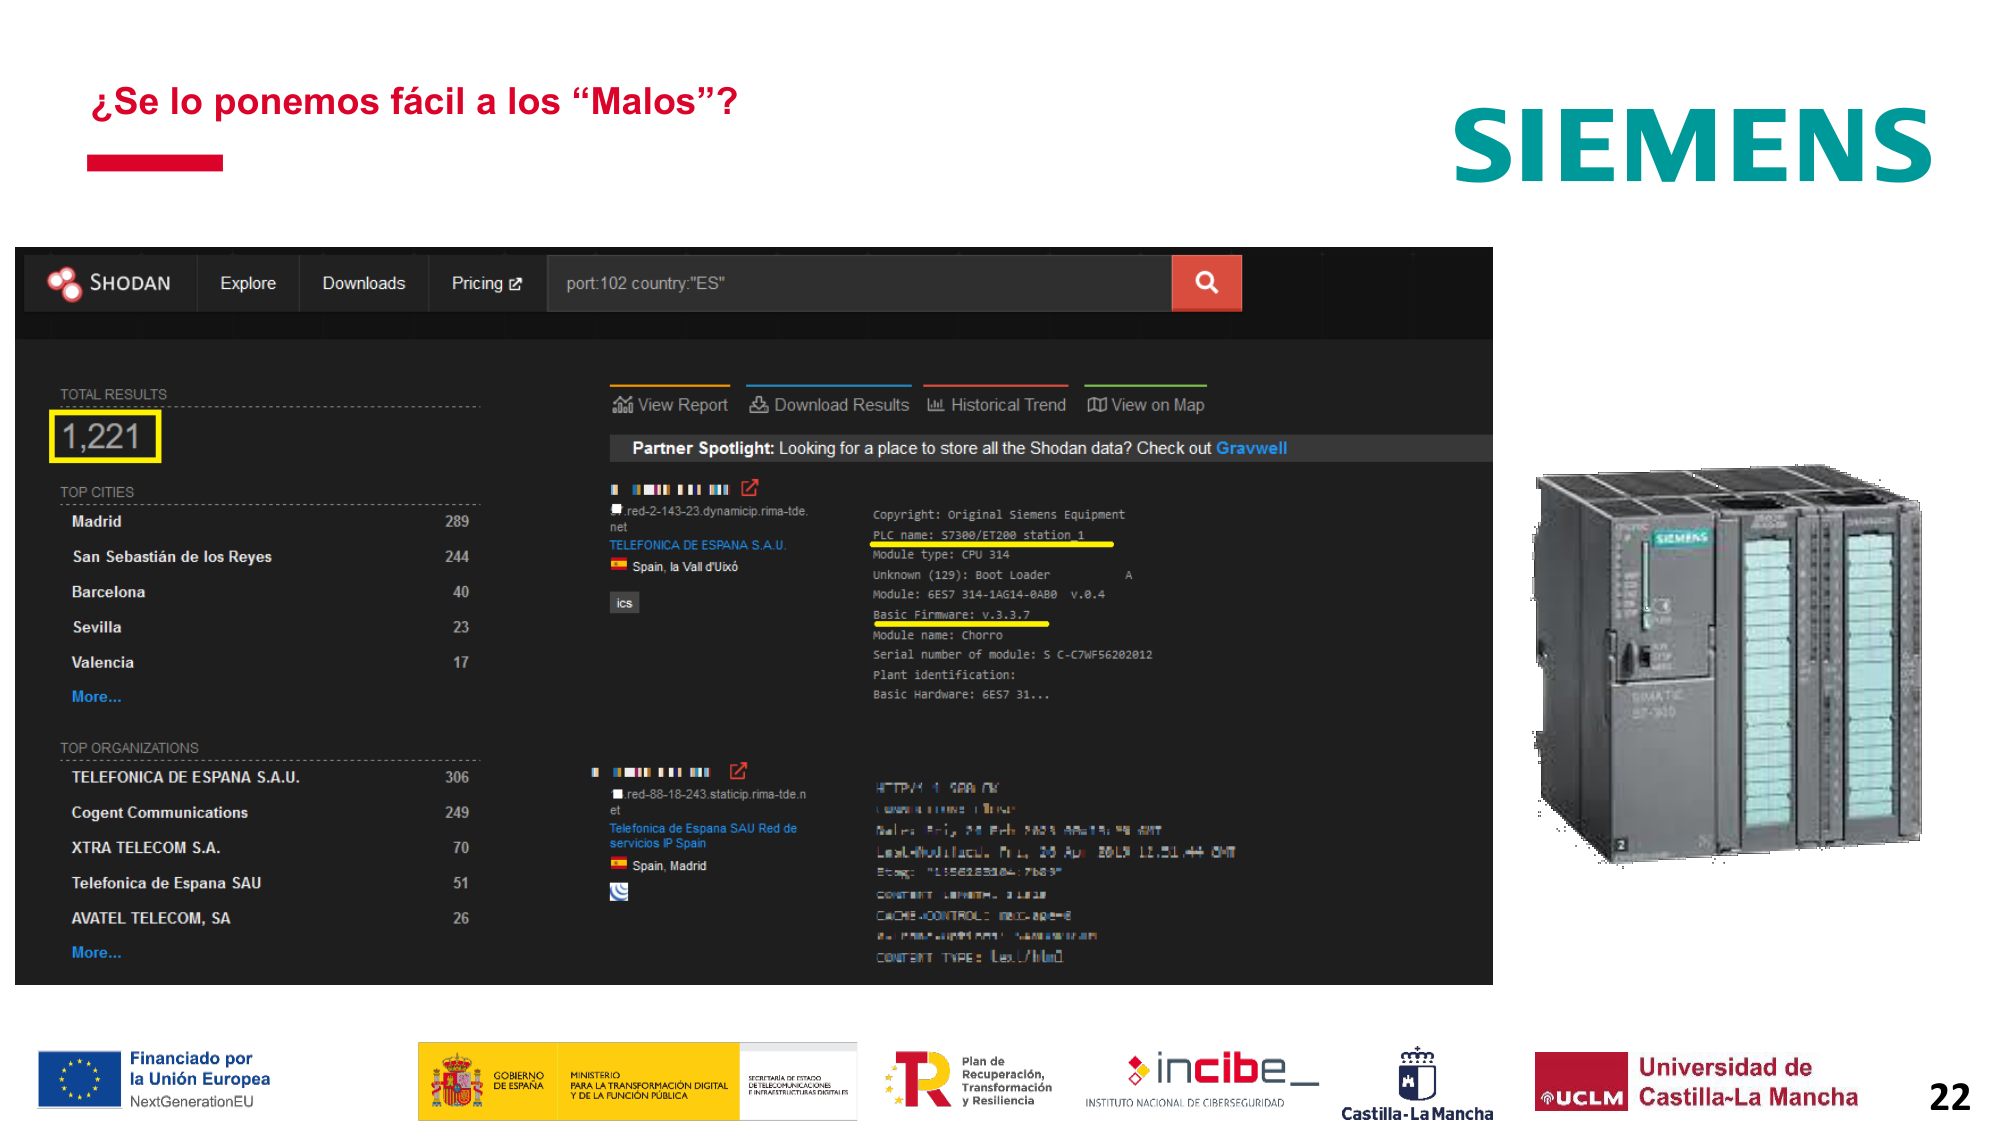
\includegraphics[trim=0 72 0 0,clip,width=\paperwidth,height=\paperheight,keepaspectratio]{img/sl010.png}
\end{frame}

\begin{frame}[allowframebreaks]{Introducción}
\small
  \begin{itemize}
  \item ¿De qué protegernos? Vectores de ataque
  \item Phishing / spear-phishing y adjuntos maliciosos.
  \item Alta exposición (digitalización, nube, Edge, Industria 4.0).
  \item Insiders, medios extraíbles, instalación de malware, accesos remotos.
  \item Manipulación de comunicaciones (MiTM) y protocolos inseguros.
  \item Vulnerabilidades: exploits, contraseñas débiles o en claro, sistemas legacy.
  \item ¿Quién los utiliza?
  \item Empleados descontentos $\cdot$ individuos / hacktivistas $\cdot$ competencia $\cdot$ grupos criminales $\cdot$ terroristas, servicios de inteligencia y Estados.
  \item Fuente: RoadMap Empresa Cibersegura
  \end{itemize}
\end{frame}

\begin{frame}[allowframebreaks]{Introducción}
\small
  Seguridad de la Información:
\begin{itemize}
  \item Conjunto de medidas preventivas y reactivas que permiten resguardar y proteger la información buscando mantener la confidencialidad, la disponibilidad e integridad de la misma
\end{itemize}
  Ciberseguridad:  
  \begin{itemize}
  \item Es ``la protección de los activos de información frente a las amenazas de la información procesada, almacenada y transportada por los sistemas de información interconectados''
  \end{itemize}
  Diferencias:
  \begin{itemize}
  \item Hay que tener claro que ciberseguridad es parte de la seguridad de la información, se refiere a la protección de activos digitales (información, hardware y redes) mientras que en la seguridad de la información, se incluye tanto activos digitales, como activos en papel
  \end{itemize}
\end{frame}

\begin{frame}[allowframebreaks]{Definiciones}
\small
  \begin{itemize}
  \item Confidencialidad
  \item Integridad
  \item Disponibilidad
  \end{itemize}
\begin{center}
\includegraphics[width=0.72\textwidth,height=0.58\textheight,keepaspectratio]{img/sl014.png}
\end{center}
\end{frame}

\section{Definiciones}

\begin{frame}{Definiciones}
\scriptsize
  Triada CIA: Ejemplos Reales de Violaciones.
\begin{itemize}
  \item Confidencialidad --- Filtración de datos Equifax (2017):
\begin{itemize}
  \item Vulnerabilidad en Apache Struts (\href{https://nvd.nist.gov/vuln/detail/CVE-2017-5638}{CVE-2017-5638}, CVSS 9.8) permitió inyectar código en el servidor
  \item $\rightarrow$ 147 millones de registros con nombre, DNI, fecha de nacimiento y n de tarjeta expuestos
  \item Referencia: \href{https://www.gao.gov/products/gao-18-559}{GAO-18-559 --- Data Protection: Actions Taken by Equifax and Federal Agencies in Response to the 2017 Breach} (informe oficial, 2018)
  \end{itemize}
  \item Integridad --- Ataque a Target (2013)
\begin{itemize}
  \item Malware BlackPOS instalado en sistemas TPV mediante credenciales de un proveedor
  \item $\rightarrow$ Datos de 40 millones de tarjetas bancarias capturados y modificados en tránsito
  \item Referencia: \href{https://krebsonsecurity.com/2014/02/target-hackers-broke-in-via-hvac-company/}{Krebs on Security --- Target Hackers Broke in Via HVAC Company} (2014)
  \end{itemize}
  \item Disponibilidad --- DDoS a Dyn (2016)
  \begin{itemize}
  \item Botnet Mirai (dispositivos IoT infectados) generó 1.2 Tbps de tráfico
  \item $\rightarrow$ Twitter, Netflix, Spotify y GitHub inaccesibles durante horas en EE.UU. y Europa
  \item Referencia: \href{https://www.usenix.org/conference/usenixsecurity17/technical-sessions/presentation/antonakakis}{Antonakakis et al. --- Understanding the Mirai Botnet}, USENIX Security 2017
  \end{itemize}
  \end{itemize}
\end{frame}

\begin{frame}[allowframebreaks]{Definiciones}
\small
Otros atributos de seguridad de la información:
  \begin{itemize}
  \item Se trata de atributos asociados a la funcionalidad de la información.
  \item Autenticidad: permite comprobar que alguien o algo es quien dice ser
  \item NO Repudio: se trata de identificar de forma biunívoca la pertenencia de una información a un individuo.
  \item Estos atributos se convierten en fundamentales en la FIRMA DIGITAL
  \item Fiabilidad: la probabilidad de que un sistema se comporte tal y como se espera de él
  \end{itemize}
\end{frame}

\begin{frame}[allowframebreaks]{Definiciones}
\small
  Daño:
  \begin{itemize}
  \item Perjuicio que se produce a raíz de un fallo en un sistema.
  \item Económico, físico, moral, etc.
  \item Fortuito o provocado.
  \end{itemize}
  Ataque:
  \begin{itemize}
  \item Acción de provocar un daño a un sistema de forma intencionada.
  \end{itemize}
  Riesgo:
  \begin{itemize}
  \item Producto entre la magnitud del daño (d) y la probabilidad de que éste ocurra Pd :
  \item R = d $\cdot$ Pd
  \item Un daño bajo pero muy probable puede suponer más riesgo que un daño mayor, aunque muy poco probable.
  \end{itemize}
\end{frame}

\begin{frame}[allowframebreaks]{Definiciones}
\small
Vulnerabilidad
  \begin{itemize}
  \item Situación de daño cuyo riesgo de producirse es significativo.
  \item Deficiencia de un sistema susceptible de producir --accidental o intencionadamente-- un fallo en el mismo. (punto débil)
  \end{itemize}
  Exploit
  \begin{itemize}
  \item Técnica que permite aprovechar una vulnerabilidad para producir un daño, y romper la seguridad de un sistema.
  \end{itemize}
\end{frame}

\begin{frame}{Definiciones}
\begin{center}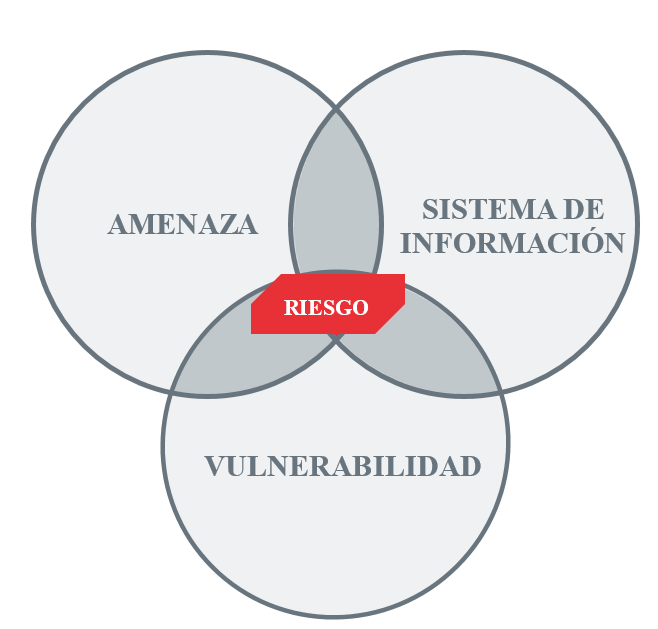
\includegraphics[width=\textwidth,height=0.92\textheight,keepaspectratio]{img/sl019.png}
\end{center}
\end{frame}

\begin{frame}{Definiciones}
\begin{center}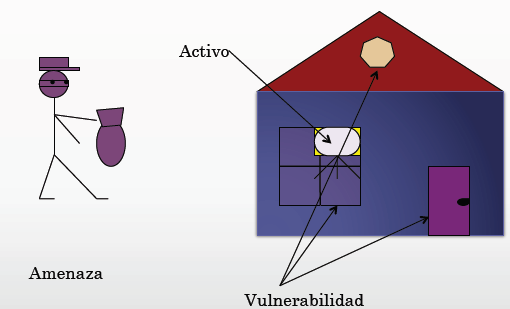
\includegraphics[width=\textwidth,height=0.92\textheight,keepaspectratio]{img/sl020.png}
\end{center}
\end{frame}

\begin{frame}{Definiciones}
\small
Payload:
  \begin{itemize}
  \item Es el resultado de un fallo de programación introducido en el proceso de creación de programas de ordenadores
  \item Parte del código de un exploit que tiene como objetivo ejecutarse en la máquina víctima para realizar la acción maliciosa
  \item Ejemplos: Meterpreter, backdoor, etc\dots{}
  \end{itemize}
\vfill
\begin{center}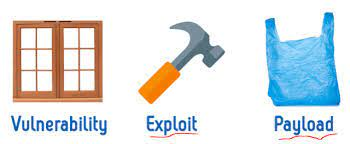
\includegraphics[width=0.62\textwidth,height=0.45\textheight,keepaspectratio]{img/sl021.jpg}
\end{center}
\end{frame}

\begin{frame}{Definiciones}
\footnotesize

¿Cómo clasificar a nivel mundial las vulnerabilidades que los distintos fabricantes van publicando?
  

  \begin{itemize}
  \item CVE: (Common Vulnerabilities and Exposures).CVE es un código asignado a una vulnerabilidad que le permite ser identificada de forma univoca. Proporcionan un identificador universal para las vulnerabilidades.
  \item Se conoce como identificador CVE (CVE-ID) y está formado por las siglas de este diccionario
  \item Elementos:
  \begin{itemize}

  \item Un número (ej: CVE-1999-0067)
  \item Estado: candidato (candidate) o definitivo (entry).
  \item Breve descripción de la vulnerabilidad.
  \item Referencias.
  \end{itemize}
  \end{itemize}
\vfill
\begin{center}
\includegraphics[width=0.62\textwidth,height=0.40\textheight,keepaspectratio]{img/sl026.png}
\end{center}
\end{frame}

\begin{frame}{Definiciones}
\begin{center}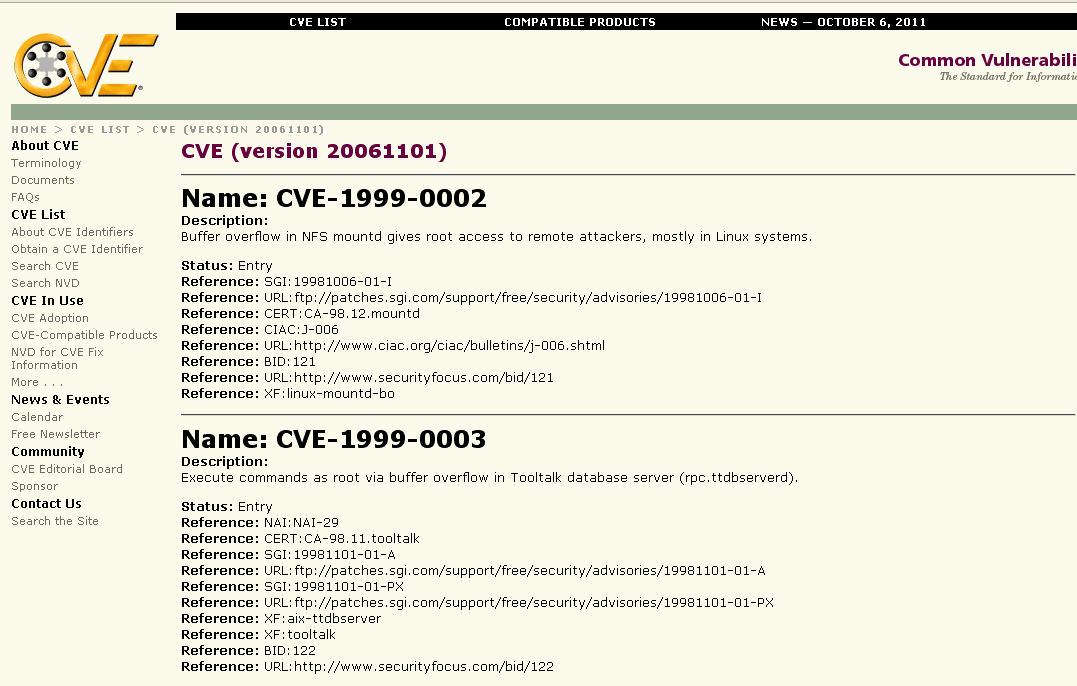
\includegraphics[width=\textwidth,height=0.92\textheight,keepaspectratio]{img/sl024.png}
\end{center}
\end{frame}

\begin{frame}[allowframebreaks]{Definiciones}
\small
  \begin{itemize}
  \item MITRE es una organización sin ánimo de lucro que gestiona los CVE. Se encarga de registrar y oficializar todos los datos relativos a vulnerabilidades, debilidades y ataques conocidos. Toda esta información es de carácter público y puede ser consultada libremente.
  \item CVE es una lista de vulnerabilidades de seguridad de la información públicamente conocidas.
  \item  Ejemplo:
  \begin{itemize}
  \item \href{https://es-la.tenable.com/blog/three-vulnerability-intelligence-insights-worth-your-attention}{Diferentes CVE de navegador web de gravedad Alta que prevalecen en entornos empresariales}
  \item \href{https://www.cvedetails.com/}{CVE Details --- base de datos de vulnerabilidades}
  \end{itemize}
    \end{itemize}
\begin{center}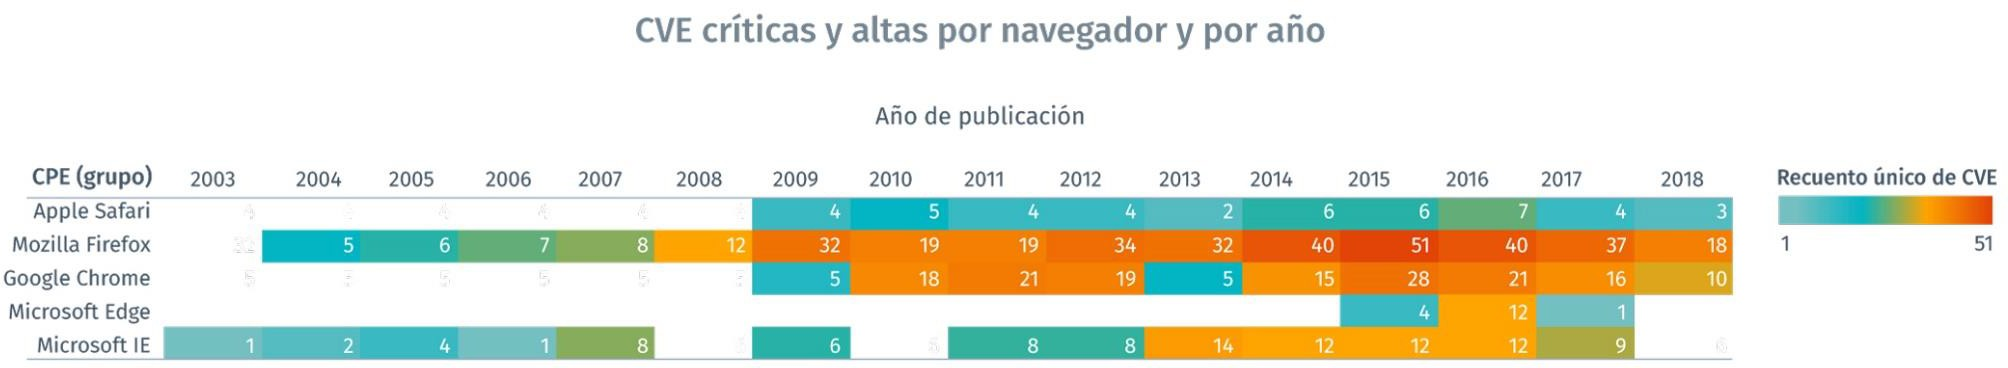
\includegraphics[width=0.72\textwidth,height=0.58\textheight,keepaspectratio]{img/sl025.jpg}
\end{center}
\end{frame}


\begin{frame}[allowframebreaks]{Definiciones}
\small
  \begin{itemize}
  \item CWE (Common Weakness Enumeration) es una lista de tipos de debilidades de software dirigida a desarrolladores y profesionales de la seguridad. Fue creada al igual que CVE para unificar la descripción de las debilidades de seguridad de software en cuanto a arquitectura, diseño y código se refiere. Se puede ver como un catálogo de debilidades documentadas que se suelen cometer programando, y que podría derivar en vulnerabilidades. CWE satisface la necesidad de conocer y tener catalogadas las distintas debilidades existentes
  \end{itemize}
\begin{center}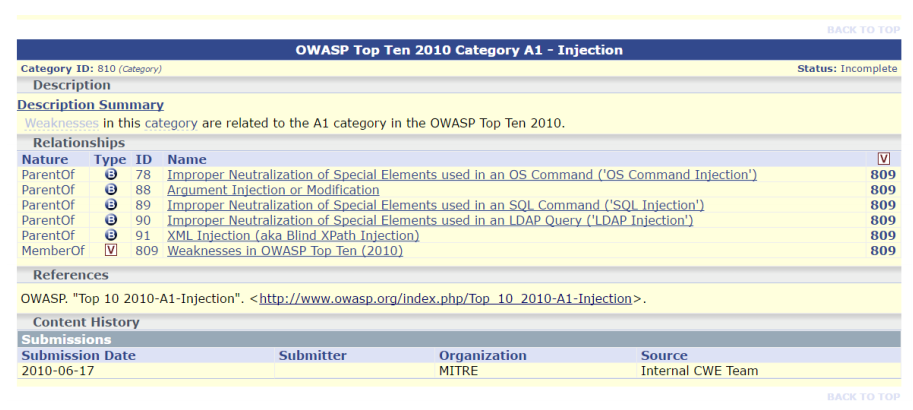
\includegraphics[width=\textwidth,height=0.92\textheight,keepaspectratio]{img/sl027.png}
\end{center}
\end{frame}

\begin{frame}[allowframebreaks]{Definiciones}
\small
  \begin{itemize}
  \item CAPEC (Common Attack Pattern Enumeration and Classification) es un catálogo de patrones de ataque que se encarga de recopilar información sobre ellos, junto a un esquema de clasificación exhaustiva. Estos patrones de ataques no son más que las descripciones de los métodos comunes utilizados para la explotación de vulnerabilidades.
  \end{itemize}
\begin{center}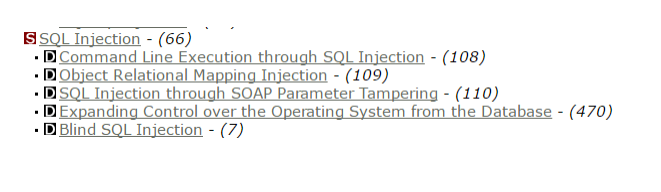
\includegraphics[width=0.72\textwidth,height=0.58\textheight,keepaspectratio]{img/sl028.png}
\end{center}
\end{frame}

\begin{frame}[allowframebreaks]{Definiciones}
\small
  \begin{itemize}
  \item Una vulnerabilidad (CVE) es explotada aprovechando a una debilidad (CWE) presente en un determinado software, que a su vez ha sido aprovechada a través de un patrón de ataque (CAPEC).
  \item \href{http://www.securityfocus.com/vulnerabilities}{http://www.securityfocus.com/vulnerabilities}
  \end{itemize}
\begin{center}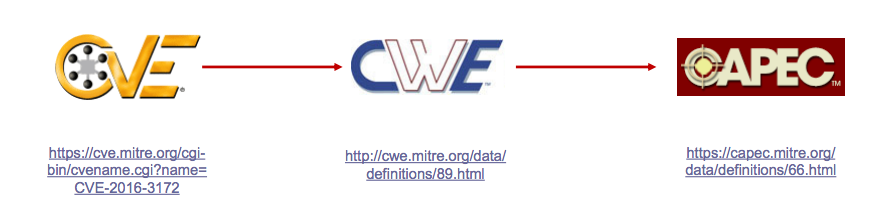
\includegraphics[width=0.72\textwidth,height=0.58\textheight,keepaspectratio]{img/sl029.png}
\end{center}
\end{frame}

\begin{frame}{Definiciones}
\small
\begin{columns}[c]
\begin{column}{0.55\textwidth}
  \begin{itemize}
  \item Una vulnerabilidad no deja de ser un bug
  \item Pero puede ser usada por un atacante con fines maliciosos
  \item Hay de distintos tipos y gravedad
  \item Shellshock-CVE-2014-6271
  \item CVSS Score 10.0
  \end{itemize}
\end{column}
\begin{column}{0.43\textwidth}
\begin{center}
\includegraphics[width=\textwidth,height=0.65\textheight,keepaspectratio]{img/sl030.png}
\end{center}
\end{column}
\end{columns}
\end{frame}

\begin{frame}{Definiciones}
\small
\begin{columns}[c]
\begin{column}{0.55\textwidth}
  \begin{itemize}
  \item ¿Cómo medimos como de peligrosa es una vulnerabilidad? CVSS (Common Vulnerability Score System)
  \item Principios CIA:
    \begin{itemize}
    \item CR, IR, AR (Confidentiality, Integrity, Availability Requirements)
    \end{itemize}
  \end{itemize}
\end{column}
\begin{column}{0.43\textwidth}
\begin{center}
\includegraphics[width=\textwidth,height=0.65\textheight,keepaspectratio]{img/sl031.png}
\end{center}
\end{column}
\end{columns}
\end{frame}

\begin{frame}[allowframebreaks]{Definiciones}
\small
  \begin{itemize}
  \item AV (Attack Vector): accesibilidad de la vulnerabilidad
    \begin{itemize}
    \item AC (Attack Complexity): condiciones fuera del control del atacante
    \item AT (Attack Requirements): recursos necesarios para el ataque
    \item PR (Privileges Required): nivel de privilegios necesarios
    \item UI (User Interaction): participación de usuario requerida
    \end{itemize}
  \item Métricas de Impacto
    \begin{itemize}
    \item VC, VI, VA (Vulnerable System Confidentiality, Integrity, Availability): impacto directo
    \item SC, SI, SA (Subsequent System Confidentiality, Integrity, Availability): impacto en sistemas conectados
    \end{itemize}
  \item Métricas temporales:
    \begin{itemize}
    \item E (Exploit Maturity): estado actual de las técnicas de explotación
    \item RL (Remediation Level): tipo y disponibilidad de la solución
    \item RC (Report Confidence): grado de confianza en la existencia de la vulnerabilidad
    \end{itemize}
  \end{itemize}
\end{frame}

\begin{frame}[allowframebreaks]{Definiciones}
\small
  \begin{itemize}
  \item CVSS: Cómo Interpretar la Puntuación
  \item El CVSS v3.1 puntúa de 0.0 a 10.0 en base a vectores objetivos:
  \begin{itemize}

  \item 0.0 $\rightarrow$ Sin riesgo
  \item 0.1 -- 3.9 $\rightarrow$ Bajo Ejemplo: bug local sin acceso a datos
  \item 4.0 -- 6.9 $\rightarrow$ Medio Ejemplo: XSS en panel de admin autenticado
  \item 7.0 -- 8.9 $\rightarrow$ Alto Ejemplo: SQLi que permite leer toda la BBDD
  \item 9.0 -- 10.0 $\rightarrow$ Crítico Ejemplo: RCE remoto sin autenticación
  \end{itemize}
    \item Casos reales por puntuación

  \begin{itemize}
  \item 10.0 --- Log4Shell (CVE-2021-44228): RCE en Log4j, sin auth, por red
  \item 9.8 --- ProxyLogon (CVE-2021-26855): RCE en Microsoft Exchange
  \item 7.5 --- Heartbleed (CVE-2014-0160): fuga de memoria en OpenSSL
  \item 6.1 --- XSS reflejado típico en aplicación web con usuario autenticado
  \end{itemize}
  \item La puntuación guía la priorización del parcheo: parchear primero los $\geq$ 9.0
\end{itemize}
\end{frame}

\begin{frame}{Ejercicio}
\small
\begin{center}
\includegraphics[width=0.55\textwidth,height=0.55\textheight,keepaspectratio]{img/sl033.jpg}
\end{center}
\vfill
  \begin{itemize}
  \item Visita la web \href{https://www.cvedetails.com/}{cvedetails} y busca una vulnerabilidad a tu elección
  \item Utiliza la \href{https://nvd.nist.gov/vuln-metrics/cvss/v3-calculator}{herramienta online} para calcular el CVSS de una vulnerabilidad
  \item Visita la web \href{https://www.exploit-db.com/}{exploitdb} para ver qué tipos de exploits hay disponibles
  \end{itemize}
\end{frame}

\begin{frame}{Definiciones}
\small
\begin{columns}[c]
\begin{column}{0.54\textwidth}
  Causas de una vulnerabilidad:
  \begin{itemize}
  \item Mal diseño del sistema.
  \item Mal configurado
  \item Implementación deficiente:
    \begin{itemize}
    \item A nivel de software: Bugs.
    \item A nivel de hardware.
    \item Reutilización de código
    \end{itemize}
  \item Un uso inadecuado:
    \begin{itemize}
    \item Un sistema puede enfrentarse a situaciones de uso para las que no está diseñado, dando lugar a vulnerabilidades.
    \end{itemize}
  \end{itemize}
\end{column}
\begin{column}{0.44\textwidth}
\begin{center}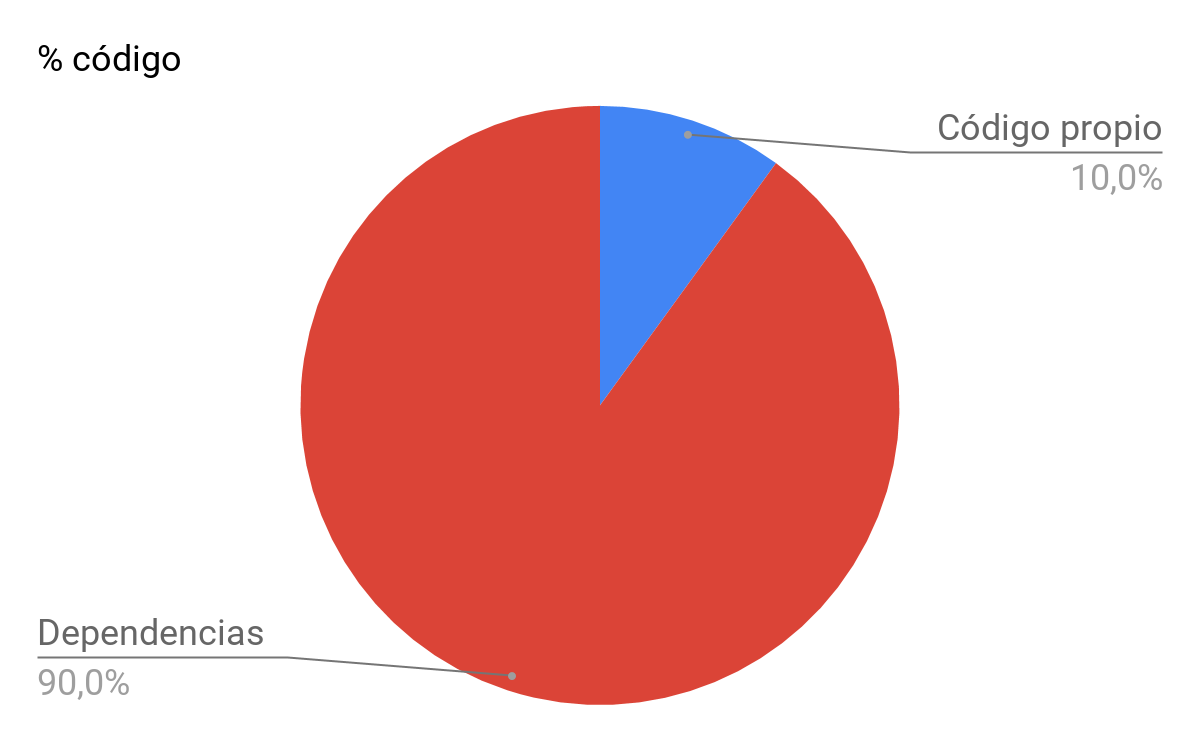
\includegraphics[width=\textwidth,height=0.72\textheight,keepaspectratio]{img/sl034.png}
\end{center}
\end{column}
\end{columns}
\end{frame}

\begin{frame}[allowframebreaks]{Definiciones}
\small
Detección:
  \begin{itemize}
  \item Ciclo Desarrollo Seguro de Software. Estudiando el sistema en las fases de diseño, implementación y uso.
  \item Fuzzers. Sometiendo al sistema a entradas de datos no estandarizadas ni en forma ni longitud
  \item Auditorias, pentesting, reversing
  \item Aprendiendo de ataques externos, a través de sistemas trampa (Honeypots).
  \item De manera fortuita. \href{https://unaaldia.hispasec.com/2021/01/ninos-jugando-encuentran-una-vulnerabilidad-en-el-salvapantallas-de-linux-mint.html}{Ejemplo}
  \end{itemize}
\end{frame}

\begin{frame}[allowframebreaks]{Definiciones}
\small
  \begin{itemize}
  \item Se estima que en torno al 99\% de los casos de intrusión son el resultado de un ataque contra vulnerabilidades conocidas o errores solucionables
  \end{itemize}
\begin{center}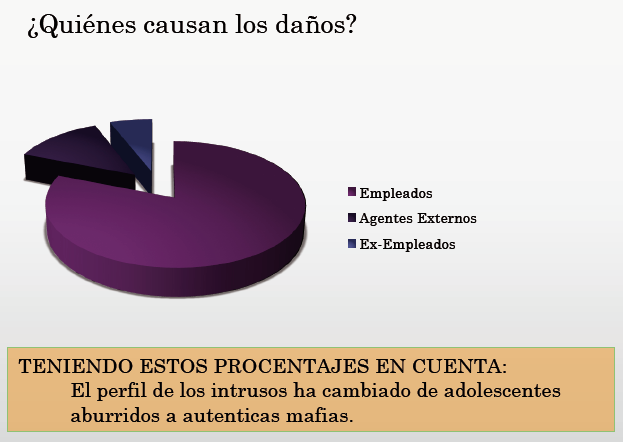
\includegraphics[width=0.72\textwidth,height=0.58\textheight,keepaspectratio]{img/sl036.png}
\end{center}
\end{frame}

\begin{frame}{Definiciones}
\footnotesize
Zero day
  \begin{itemize}
  \item Vulnerabilidad que es desconocido por la comunidad y el fabricante del producto.
  \item Ventana de Exposición
    \begin{itemize}
    \item Tiempo que transcurre desde que se detecta hasta que ésta se corrige.
    \item Durante este tiempo, el sistema está sujeto a una amenaza.
    \item Hay que intentar que la ventana de exposición sea lo más pequeña posible.
    \end{itemize}
  \end{itemize}
\vfill
\begin{center}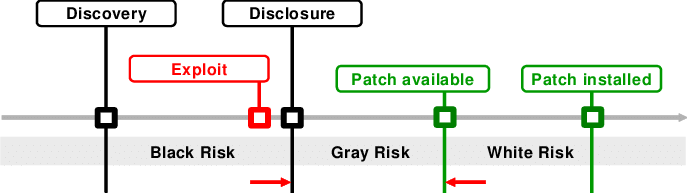
\includegraphics[width=0.82\textwidth,height=0.45\textheight,keepaspectratio]{img/sl037.png}
\end{center}
\end{frame}

\begin{frame}{Definiciones}
  Proceso de descubrir y publicar una vulnerabilidad
\begin{center}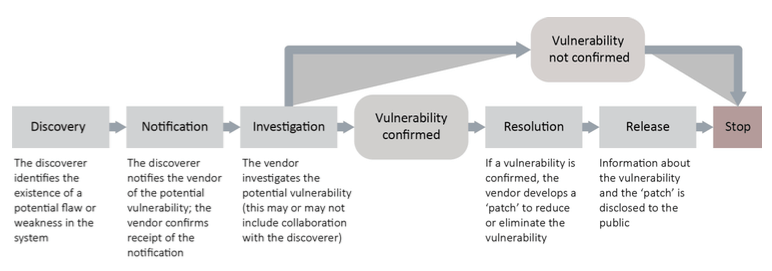
\includegraphics[width=\textwidth,height=0.92\textheight,keepaspectratio]{img/sl038.png}
\end{center}
\end{frame}

\begin{frame}[allowframebreaks]{Definiciones}
\small
Zero Day: Casos Históricos Relevantes
\begin{itemize}
  \item Stuxnet (2010) --- CVE-2010-2568 [CVSS 9.3]
\begin{itemize}
  \item Primer ciberarma conocida: saboteó centrifugadoras de uranio en Natanz, Irán
  \item Usó 4 zero-days simultáneos en Windows + vulnerabilidades en PLCs Siemens
\end{itemize}

  \item Log4Shell (2021) --- CVE-2021-44228 [CVSS 10.0]

  \begin{itemize}

  \item RCE sin autenticación en Log4j (librería Java usada en millones de apps)
  \item Afectó a Apple, Amazon, Tesla, Steam; explotada activamente en pocas horas
  \end{itemize}

    \item EternalBlue (2017) --- CVE-2017-0144 [CVSS 8.1]
  \begin{itemize}


  \item Exploit de la NSA filtrado por Shadow Brokers; usó protocolo SMBv1 de Windows
  \item Fue la base de WannaCry: 300.000 sistemas cifrados en 150 países en 72 h
  \item $\rightarrow$ El NHS (sanidad del Reino Unido) canceló 19.000 citas médicas por el ataque
  \end{itemize}

\end{itemize}
\end{frame}

\begin{frame}{Ejercicio}
\small
\begin{center}
\includegraphics[width=0.55\textwidth,height=0.55\textheight,keepaspectratio]{img/sl040.jpg}
\end{center}
\vfill
  \begin{itemize}
  \item Identifica una vulnerabilidad crítica o 0day
    \begin{itemize}
    \item \href{https://www.linkedin.com/posts/factum-es_ciberseguridad-windows-rce-activity-7229449975024222208-qZv4}{Ejemplo}:
    \end{itemize}
  \item Para estar al tanto de noticias y vulnerabilidades:
    \begin{itemize}
    \item \href{https://unaaldia.hispasec.com/}{https://unaaldia.hispasec.com/}
    \end{itemize}
  \end{itemize}
\end{frame}

\begin{frame}{Definiciones}
\begin{center}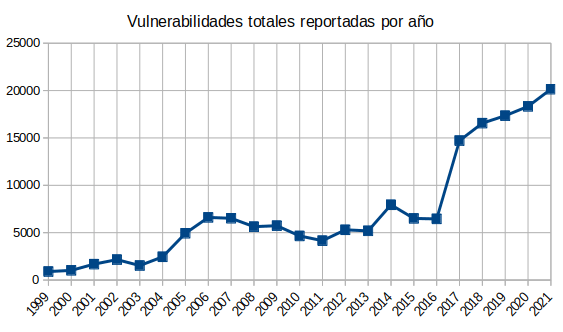
\includegraphics[width=\textwidth,height=0.92\textheight,keepaspectratio]{img/sl041.png}
\end{center}
\end{frame}

\begin{frame}{Definiciones}
\small
Gestión de los Incidentes de Seguridad:
\begin{columns}[c]
\begin{column}{0.72\textwidth}
  \begin{itemize}
  \item Grupos dedicados a estudiar vulnerabilidades y proporcionar servicios a entidades que han sido atacadas, así como divulgar avisos de seguridad.
  \item Detectar, identificar y analizar los incidentes de seguridad
  \item Desarrollar Planes de respuesta y recuperación
  \item Realizar test periódicos de los planes
  \item Documentar y Aprender del incidente
  \item A nivel nacional:
  \end{itemize}
\end{column}
\begin{column}{0.26\textwidth}
\begin{center}
\includegraphics[width=\textwidth,height=0.5\textheight,keepaspectratio]{img/sl042.png}
\end{center}
\end{column}
\end{columns}
\end{frame}

\begin{frame}{Definiciones}
\small
\begin{columns}[c]
\begin{column}{0.68\textwidth}
  \begin{itemize}
  \item Hacker:
    \begin{itemize}
  \item Persona que utiliza los ordenadores como reto intelectual, con amplios conocimientos informáticos
  \item Amplios conocimientos en tecnología, informática, electrónica o comunicaciones
  \item Se mantiene permanentemente actualizado y conoce a fondo todo lo relacionado con la tecnología y sistemas y conoce las debilidades. En general, buscan información sin causar daño.
  \item Hacker Ético != Pirata informático / Cibercriminal
  \item El Hacking es el ARTE de hacer que las cosas funcionen de manera diferente a como su creador originalmente pensó.
  \end{itemize}
  \end{itemize}
\end{column}
\begin{column}{0.30\textwidth}
\begin{center}
\includegraphics[width=\textwidth,height=0.55\textheight,keepaspectratio]{img/sl043.png}
\end{center}
\end{column}
\end{columns}
\end{frame}

\begin{frame}{Definiciones}
\small
\begin{columns}[c]
\begin{column}{0.68\textwidth}
\begin{itemize}
\item Cracker / Ciberciminal:
 \begin{itemize}
  \item Persona que utiliza ordenadores ajenos para cometer Delitos
    \item Comportamiento compulsivo: alardea de su capacidad para reventar sistemas electrónicos e informáticos. Es malicioso.
    \item Es un hacker con fines no éticos
    \end{itemize}
  \item Script kiddie
    \begin{itemize}
    \item Usuario de informática no experto que rompe la seguridad de un sistema usando exploits.
    \item se limitan a recopilar información de la red y a buscar programas que luego ejecutan sin los más mínimos conocimientos
    \end{itemize}
  \end{itemize}
\end{column}
\begin{column}{0.30\textwidth}
\begin{center}
\includegraphics[width=\textwidth,height=0.55\textheight,keepaspectratio]{img/sl044.jpg}
\end{center}
\end{column}
\end{columns}
\end{frame}

\begin{frame}[allowframebreaks]{Definiciones}
\small

  \begin{itemize}
    \item Lammer
     \begin{itemize}
  \item Similar a script kiddie
    \end{itemize}

  \item Copyhacker
    \begin{itemize}
  \item Falsificadores dedicados al crackeo de Hardware, específicamente en el sector de tarjetas inteligentes en televisiones de pago
    \end{itemize}

  \item Phreaker
     \begin{itemize}
  \item Se caracterizan por poseer vastos conocimientos en el área de telefonía terrestre y móvil, incluso más que los propios técnicos de las compañías telefónicas
      \end{itemize}

  \item Hacktivist
    \begin{itemize}
  \item Hacker que utiliza la tecnología para reivindicar sus ideas (sociales, políticas, etc.). Por ejemplo Anonymous.
    \end{itemize}

  \end{itemize}
\end{frame}

\begin{frame}[allowframebreaks]{Definiciones}
\small
Advanced Persistent Threats (APTs)
  \begin{itemize}
  \item Es un conjunto de procesos informáticos sigilosos orquestados por un tercero con la intención y la capacidad de atacar de forma avanzada (a través de múltiples vectores de ataque) y continuada en el tiempo, un objetivo determinado (normalmente, gobiernos, empresas grandes, etc)
  \item La intrusión suele llevar el despliegue de un malware, que es instalado usando exploits que aprovechan vulnerabilidades de día 0 del objetivo.
  \item Mapa de organizaciones:
    \begin{itemize}
    \item \href{https://attack.mitre.org/groups/}{MITRE ATT\&CK --- Groups}: catálogo de grupos APT con sus alias por fabricante, la organización a la que se atribuyen y sus técnicas documentadas
    \item \href{https://apt.etda.or.th/cgi-bin/aptgroups.cgi}{Threat Group Cards (ETDA)}: enciclopedia de actores, buscable por país de origen y sector objetivo
    \item Caso fundacional: \href{https://www.mandiant.com/resources/reports/apt1-exposing-one-chinas-cyber-espionage-units}{Mandiant --- APT1: Exposing One of China's Cyber Espionage Units} (2013), que atribuyó APT1 a la Unidad 61398 del Ejército Popular de Liberación
    \end{itemize}
  \end{itemize}
\end{frame}

\begin{frame}[allowframebreaks]{Definiciones}
\small
  APT: Grupos Conocidos y Ataques Reales

  \begin{itemize}
  \item APT28 'Fancy Bear' --- Rusia (GRU)
  \begin{itemize}

  \item Hackeo del DNC (Partido Demócrata, EE.UU.) durante la campaña electoral de 2016
  \item Técnicas: spear phishing, robo de credenciales OAuth, uso de 0-days en Office
  \end{itemize}
  \item APT41 'Double Dragon' --- China

  \begin{itemize}

  \item Ataca con motivación mixta: espionaje estatal + beneficio económico (ransomware)
  \item Comprometió empresas farmacéuticas durante el desarrollo de vacunas COVID-19
    \end{itemize}
  \item Lazarus Group --- Corea del Norte
  \begin{itemize}

  \item Robó 81 M\$ al Banco Central de Bangladesh mediante transferencias SWIFT falsas
  \item Ataque a Sony Pictures (2014): 100 TB robados, sistemas destruidos con wiper
  \item   \end{itemize}
  \item $\rightarrow$ Patrón común: recursos ilimitados, sigilo, persistencia y motivación estratégica
  \end{itemize}
\end{frame}

\begin{frame}[allowframebreaks]{Definiciones}
\small
MITRE ATT \& CK\textregistered{}
  \begin{itemize}
  \item Es una base de conocimiento accesible a nivel mundial de tácticas, procedimientos y técnicas adversas basadas en observaciones del mundo real. La base de conocimientos de ATT \& CK se utiliza como base para el desarrollo de modelos y metodologías de amenazas específicas en la comunidad de productos y servicios de ciberseguridad.
  \item \href{https://attack.mitre.org/\#}{ATT \& CK} está abierto y disponible para cualquier persona u organización.
  \item Reciéntemente, también han publicado la perspectiva en defensa (blue) denominada \href{https://d3fend.mitre.org/}{d3fend}
  \end{itemize}
\end{frame}

\section{Legislación}

\begin{frame}[allowframebreaks]{Legislación}
\small
Esquema Nacional de Seguridad
  \begin{itemize}
  \item Establece la política de seguridad en la utilización de medios electrónicos
  \item Constituido por principios básicos y requisitos mínimos
  \item Objetivos:
    \begin{itemize}
    \item Crear las condiciones necesarias de confianza en el uso de los medios electrónicos
    \item Establecer la política de seguridad en la utilización de medios electrónicos
    \item Introducir los elementos comunes que han de guiar la actuación de las Administraciones públicas
    \item Aportar un lenguaje común para facilitar la interacción de las Administraciones públicas
    \item Aportar un tratamiento homogéneo de la seguridad
    \item Facilitar un tratamiento continuado de la seguridad.
    \end{itemize}
  \end{itemize}
\end{frame}

\begin{frame}{Legislación}
\begin{center}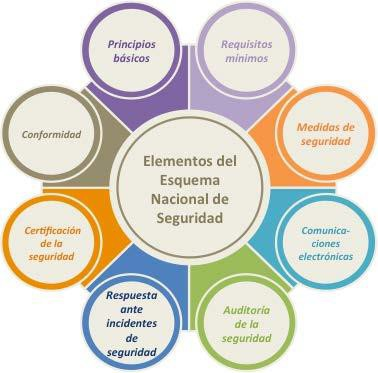
\includegraphics[width=\textwidth,height=0.92\textheight,keepaspectratio]{img/sl056.jpg}
\end{center}
\end{frame}

\begin{frame}[allowframebreaks]{Legislación}
\small
  \begin{itemize}
  \item Los estándares dan estructura
  \item Marcos y normas guían la seguridad: ISO 27001 (gestión, ya visto), el ENS, y en el mundo industrial, ISA/IEC 62443.
  \item ISA/IEC 62443 organiza la seguridad de los sistemas industriales (IACS) en 4 grupos:
  \item General $\cdot$ Políticas y procedimientos $\cdot$ Sistema (zonas y conductos) $\cdot$ Componentes (producto).
  \item Idea transferible: separar terminología, gestión, arquitectura y producto sirve para cualquier programa de seguridad.
  \item Fuente: ISA/IEC 62443
  \end{itemize}
\end{frame}

\begin{frame}[allowframebreaks]{Legislación}
\small
Normativa: Directiva NIS2
  \begin{itemize}
  \item La regulación europea más completa
  \item NIS2 obliga a muchas organizaciones (energía, salud, transporte, banca, agua, digital\dots{}) a gestionar riesgos y notificar incidentes.
  \item Cifras: +160.000 organizaciones afectadas $\cdot$ hasta 10 M\euro{} de multa $\cdot$ 15 sectores cubiertos.
  \item Hitos: en vigor 2023; transposición de los Estados el 17-oct-2024; lista de entidades esenciales/importantes en 2025.
  \item El reporte de incidentes se canaliza por la Plataforma Nacional de Ciberseguridad.
  \item Fuente: Directiva NIS2
  \end{itemize}
\end{frame}

\section{Perfiles profesionales y certificaciones}

\begin{frame}{Perfiles profesionales y certificaciones}
\small
Junta Directiva (Board of Directors)
\begin{columns}[c]
\begin{column}{0.56\textwidth}
  \begin{itemize}
  \item Equipo de dirección (Executive Committee)
  \item Se apoyan en el responsable de seguridad de la información (Chief Information Security Officer o CISO) o en el caso de no existir, se apoyan en el gerente de seguridad de la información de mayor nivel
  \item Establece la preocupación en la gestión de la seguridad cibernética dentro de la organización
  \end{itemize}
\end{column}
\begin{column}{0.42\textwidth}
\begin{center}
\includegraphics[width=\textwidth,height=0.72\textheight,keepaspectratio]{img/sl065.jpg}
\end{center}
\end{column}
\end{columns}
\end{frame}

\begin{frame}[allowframebreaks]{Perfiles profesionales y certificaciones}
\small
  \begin{itemize}
  \item CISO, aunque en algunas organizaciones prefieren el término Chief Security Officer (CSO), responsable de todos los asuntos de seguridad, tanto físicos como digitales.
  \item Pueden variar sustancialmente entre las organizaciones.
  \end{itemize}
\begin{center}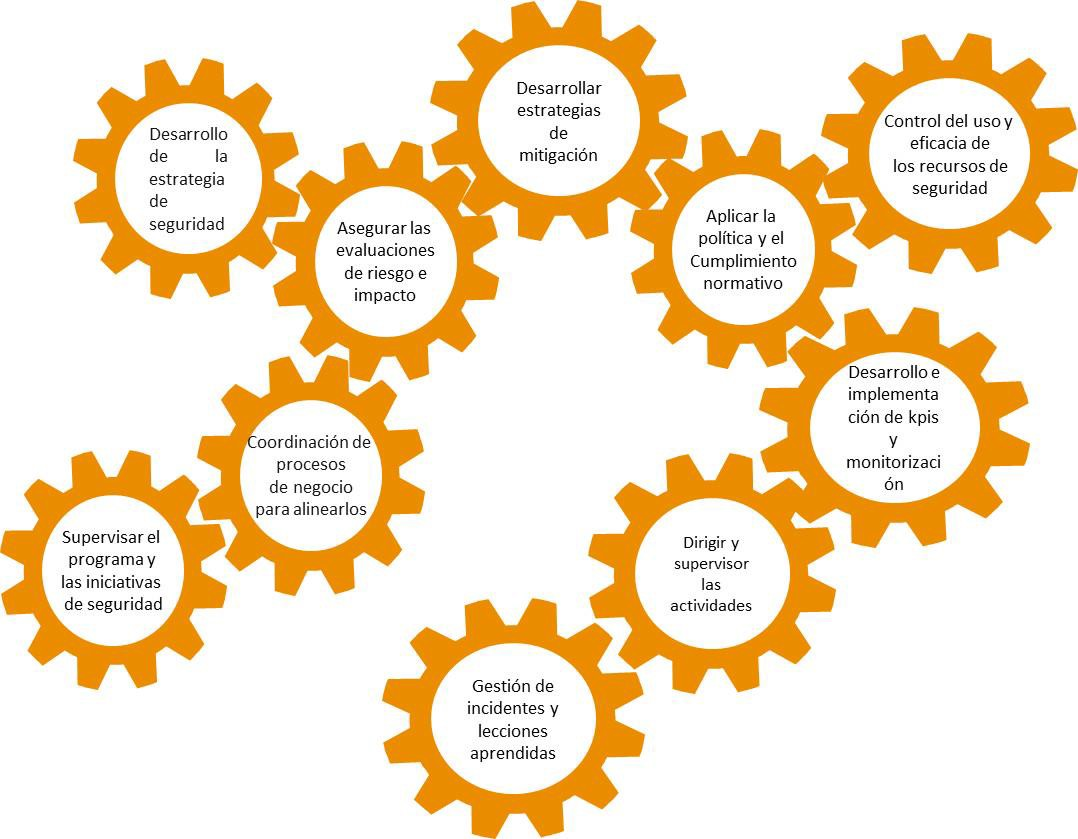
\includegraphics[width=0.72\textwidth,height=0.58\textheight,keepaspectratio]{img/sl066.jpg}
\end{center}
\end{frame}

\begin{frame}[allowframebreaks]{Perfiles profesionales y certificaciones}
\small
  \begin{itemize}
  \item Equipo de expertos en la materia, en los que se incluyen arquitectos, administradores de seguridad, analistas forenses y especialistas en seguridad de red.
  \item Diseñan, implementan y gestionan los procesos y controles técnicos
  \item Responden a los eventos e incidentes que puedan ocurrir.
  \item Trabajan dentro de la dirección, las políticas, directrices, mandatos y reglamentos establecidos por la junta de directiva, los ejecutivos y la gerencia de seguridad
  \end{itemize}
\end{frame}

\begin{frame}{Perfiles profesionales y certificaciones}
Ramas y Salidas Profesionales
  \begin{center}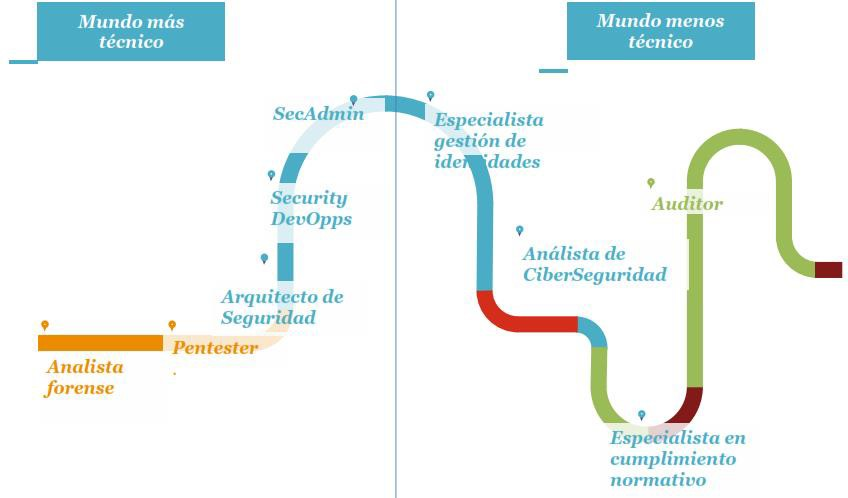
\includegraphics[width=\textwidth,height=0.92\textheight,keepaspectratio]{img/sl068.jpg}
\end{center}
\end{frame}

\begin{frame}{Perfiles profesionales y certificaciones}
\small
\begin{columns}[t]
\begin{column}{0.48\textwidth}
\begin{center}
Pentester\\[0.5ex]
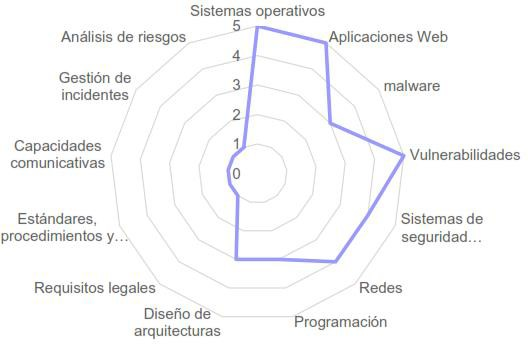
\includegraphics[width=\textwidth,height=0.72\textheight,keepaspectratio]{img/sl069.jpg}
\end{center}
\end{column}
\begin{column}{0.48\textwidth}
\begin{center}
Arquitecto de Seguridad / Security DevOps\\[0.5ex]
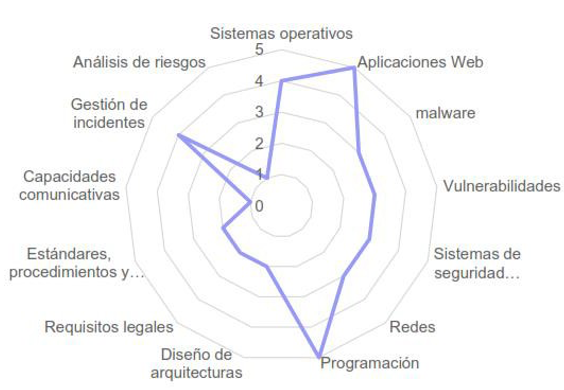
\includegraphics[width=\textwidth,height=0.72\textheight,keepaspectratio]{img/sl070.png}
\end{center}
\end{column}
\end{columns}
\end{frame}

\begin{frame}{Perfiles profesionales y certificaciones}
\small
\begin{columns}[t]
\begin{column}{0.48\textwidth}
\begin{center}
Sec-Admin / Gestión de Identidades\\[0.5ex]
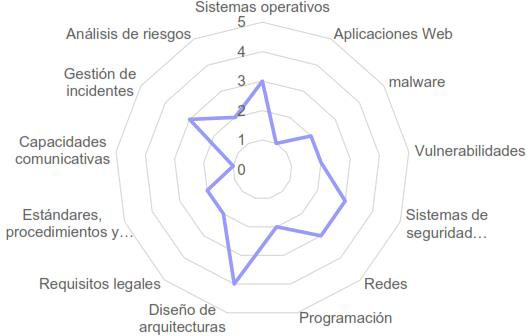
\includegraphics[width=\textwidth,height=0.72\textheight,keepaspectratio]{img/sl071.jpg}
\end{center}
\end{column}
\begin{column}{0.48\textwidth}
\begin{center}
Analista de Ciberseguridad / Cumplimiento Normativo\\[0.5ex]
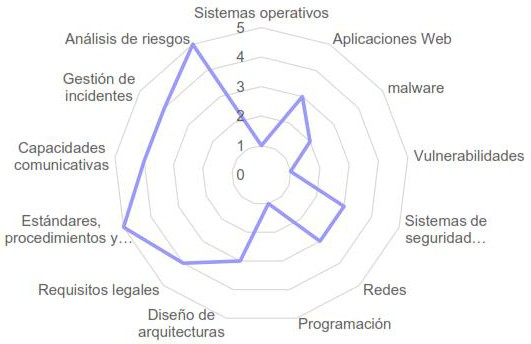
\includegraphics[width=\textwidth,height=0.72\textheight,keepaspectratio]{img/sl072.jpg}
\end{center}
\end{column}
\end{columns}
\end{frame}

\begin{frame}{Perfiles profesionales y certificaciones}
\begin{center}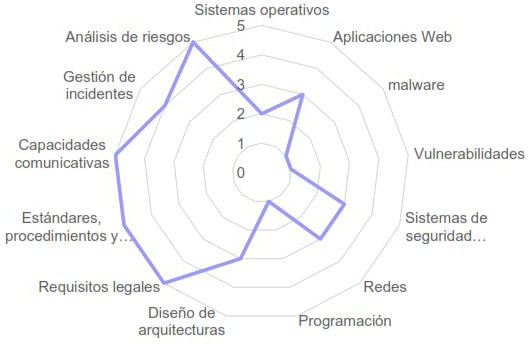
\includegraphics[width=\textwidth,height=0.92\textheight,keepaspectratio]{img/sl073.jpg}
\end{center}
\end{frame}

\begin{frame}{Perfiles profesionales y certificaciones}
\begin{center}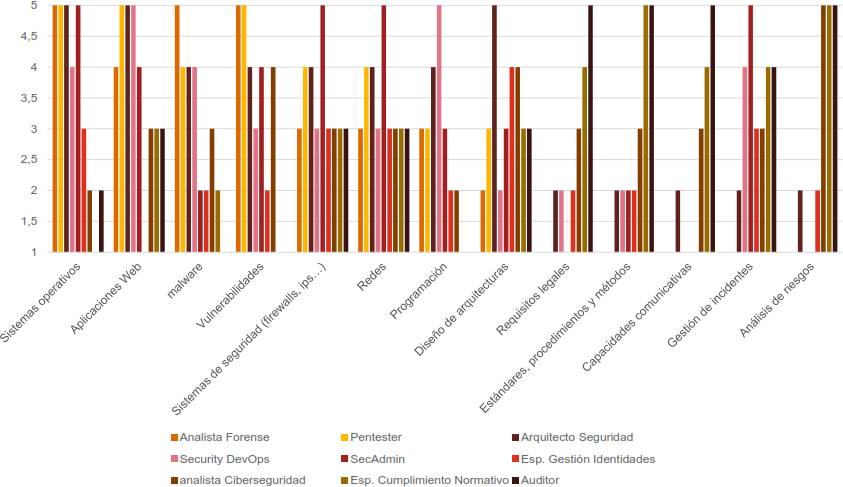
\includegraphics[width=\textwidth,height=0.92\textheight,keepaspectratio]{img/sl074.png}
\end{center}
\end{frame}

\begin{frame}[allowframebreaks]{Perfiles profesionales y certificaciones}
\small
El orden de certificaciones que la\dots{}
  \begin{itemize}
  \item El orden de certificaciones que la comunidad recomienda es: CPHE < CHEE < CEH < eJPT < eCPPT < OSWP < OSCP < eWPT < eWPTXv2 < OSCE < OSEE < OSEP < OSED
  \end{itemize}
\end{frame}

\section{El proceso de la seguridad}

\begin{frame}[allowframebreaks]{El proceso de la seguridad}
\small
La Seguridad total no existe
  \begin{itemize}
  \item Eugene Spafford, profesor de ciencias informáticas en la Universidad Purdue (Indiana, EEUU) y experto en seguridad de datos, dijo que
  \item ``el único sistema seguro es aquel que está apagado y desconectado, enterrado en un refugio de cemento, rodeado por gas venenoso y custodiado por guardianes bien pagados y muy bien armados. Aún así, yo no apostaría mi vida por él''
  \item No existe un sistema seguro o inseguro, lo que es seguro o inseguro es su funcionamiento.
  \item Un producto siempre es inseguro ya que desconocemos sus vulnerabilidades y riesgos cuando se empieza a utilizar.
  \item La seguridad no puede entenderse como un producto, sino como un proceso que debe estar presente en todas las fases del ciclo de vida de un sistema: (No es un producto cerrado)
  \end{itemize}
\end{frame}

\begin{frame}{El proceso de la seguridad}
\small
La Seguridad de la información es un camino, no es un destino.
\begin{columns}[c]
\begin{column}{0.68\textwidth}
  \begin{itemize}
  \item Modelo PDCA
    \begin{itemize}
    \item La organización debe plantearse un Sistema de Gestión de la Seguridad de la Información (SGSI), conjunto de políticas de administración de la información.
    \item El objetivo de un SGSI es proteger la información y para ello lo primero que debe hacer es identificar los 'activos de información' que deben ser protegidos y en qué grado.
    \end{itemize}
  \item Se entiende la seguridad como un proceso que nunca termina ya que los riesgos nunca se eliminan, pero se pueden gestionar. De los riesgos se desprende que los problemas de seguridad no son únicamente de naturaleza tecnológica, y por ese motivo nunca se eliminan en su totalidad.
  \end{itemize}
\end{column}
\begin{column}{0.30\textwidth}
\begin{center}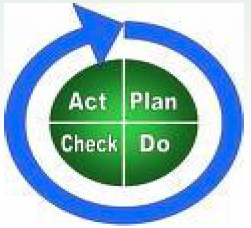
\includegraphics[width=\textwidth,height=0.6\textheight,keepaspectratio]{img/sl081.png}
\end{center}
\end{column}
\end{columns}
\end{frame}

\begin{frame}[allowframebreaks]{El proceso de la seguridad}
\small
Lecturas:
  \begin{itemize}
  \item \href{https://www.incibe-cert.es/blog/tu-empresa-segura-medir-el-primer-paso-conseguirlo}{¿Tu empresa es segura? Medir es el primer paso para conseguirlo}
  \item \href{https://www.incibe.es/extfrontinteco/img/File/intecocert/sgsi/img/Guia_apoyo_SGSI.pdf}{Implantación de un SGSI en la empresa}
  \item \href{https://www.ccn-cert.cni.es/seguridad-al-dia/comunicados-ccn-cert/4816-requisitos-minimos-de-los-sistemas-que-manejan-informacion-clasificada.html}{Requisitos mínimos de los sistemas que manejan información clasificada}
  \item \href{https://youtu.be/knxhzpNFWGI}{Análisis de Riesgos}
  \end{itemize}
\end{frame}

\begin{frame}{El proceso de la seguridad}
\small
¿Qué es la Política de Seguridad?
\begin{columns}[c]
\begin{column}{0.55\textwidth}
  \begin{itemize}
  \item Un conjunto de documentos, con un orden y una sistematización que indican normas, procedimientos y actuaciones que se deben cumplir en la Entidad.
  \item La política de seguridad establece:
    \begin{itemize}
    \item qué se protege y por qué
    \item quién es responsable de esa protección
    \item cómo resolver problemas derivados de su aplicación
    \end{itemize}
  \item La política de seguridad del sistema:
    \begin{itemize}
    \item debe ser impulsada por la administración de la empresa/institución
    \item debe ser conocida y comprendida por todos los usuarios
    \end{itemize}
  \end{itemize}
\end{column}
\begin{column}{0.43\textwidth}
\begin{center}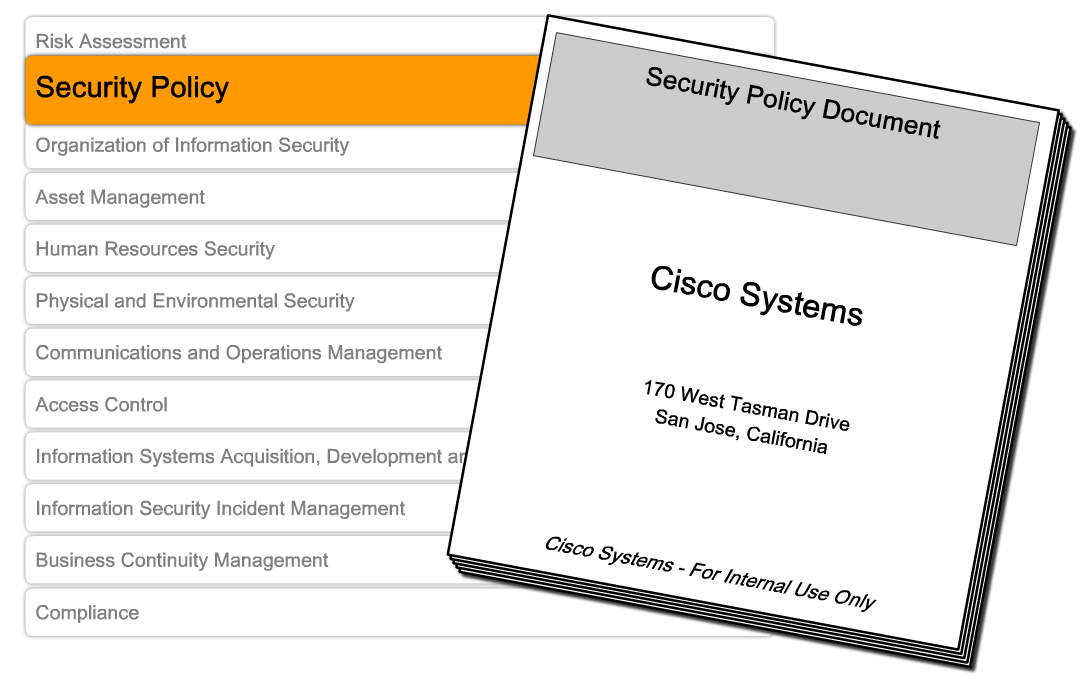
\includegraphics[width=\textwidth,height=0.75\textheight,keepaspectratio]{img/sl089.png}
\end{center}
\end{column}
\end{columns}
\end{frame}

\begin{frame}{El proceso de la seguridad}
\footnotesize
Política de Seguridad Vs. Plan de implementación
  \begin{itemize}
  \item Consiste en un estudio y análisis pormenorizado de las áreas que componen la organización que se plasma en un documento y que nos servirá para establecer una política de recuperación ante un desastre.
  \item Además de aumentar su seguridad con un plan seguridad, estratégico la empresa también gana en el conocimiento de sus fortalezas y sus debilidades.
  \item Pero si no lo hace, se expone a sufrir una pérdida irreparable mucho más costosa que la implantación de este plan
  \end{itemize}
\vfill
\begin{center}
\includegraphics[width=0.8\textwidth,height=0.45\textheight,keepaspectratio]{img/sl090.png}
\end{center}
\end{frame}

\begin{frame}{El proceso de la seguridad}
\footnotesize
Qué es la Norma ISO UNE-ISO/IEC 27001:2013 (serie 27000: marco para la gestión de la seguridad)
\begin{columns}[c]
\begin{column}{0.74\textwidth}
  \begin{itemize}
  \item Es un Sistema de Gestión que comprende:
    \begin{itemize}
    \item Política de Seguridad
    \item Estructura Organizativa
    \item Procedimientos
    \item Recursos
    \end{itemize}
  \item Es una norma que plantea un sistema de gestión que permite asegurar las continuidad de las operaciones en la organización.
  \item SGSI: proceso sistemático, documentado y conocido por toda la organización para garantizar que la seguridad de la información es gestionada correctamente
  \item ¿Qué es un Plan de Contingencia?
    \begin{itemize}
    \item es el documento que define qué hace la organización cuando el incidente ya ha ocurrido: cómo seguir operando durante la interrupción y cómo volver a la normalidad. Es la cara reactiva de la seguridad, frente a la política de seguridad, que es la cara preventiva y normativa
    \end{itemize}
  \end{itemize}
\end{column}
\begin{column}{0.24\textwidth}
\begin{center}
\includegraphics[width=\textwidth,height=0.5\textheight,keepaspectratio]{img/sl091.png}
\end{center}
\end{column}
\end{columns}
\end{frame}

\begin{frame}[allowframebreaks]{El proceso de la seguridad}
\small
RoadMap a la ciberresiliencia:
  \begin{itemize}
  \item De organización insegura a organización segura
  \item Un camino por fases para gestionar la ciberseguridad de cualquier organización:
  \begin{itemize}
  \item 1) Diagnóstico inicial 
  \item 2) Apoyo de la alta gerencia
  \item 3) Objetivos y alcance 
  \item 4) Marco de referencia.
  \item 5) Organizar la implementación 
  \item 6) Análisis y gestión de riesgos 
  \item 7) Despliegue de controles 
  \item 8) Capacitación y concienciación.
  \end{itemize}
  \item Meta: una organización resiliente con capacidad de detección y respuesta (SOC).
  
  \end{itemize}
\end{frame}

\begin{frame}[allowframebreaks]{El proceso de la seguridad}
\small
El SOC: detección y respuesta
  \begin{itemize}
  \item Vigilancia centralizada
  \item Un SOC (Centro de Operaciones de Seguridad) detecta y responde a incidentes de forma centralizada, con SIEM + SOAR.
  \item Defensa por capas: la red se segmenta en niveles (aquí el modelo Purdue, IT+OT: de los equipos de campo a la red corporativa) con cortafuegos y DMZ entre ellos.
  \item Matices por entorno
  \item En OT prima la DISPONIBILIDAD y hay mucho legacy $\rightarrow$ se detecta por tráfico de red; en IT pesa más la confidencialidad. Un SOC holístico cubre ambos.
  \end{itemize}
\end{frame}

\begin{frame}[plain]
\centering
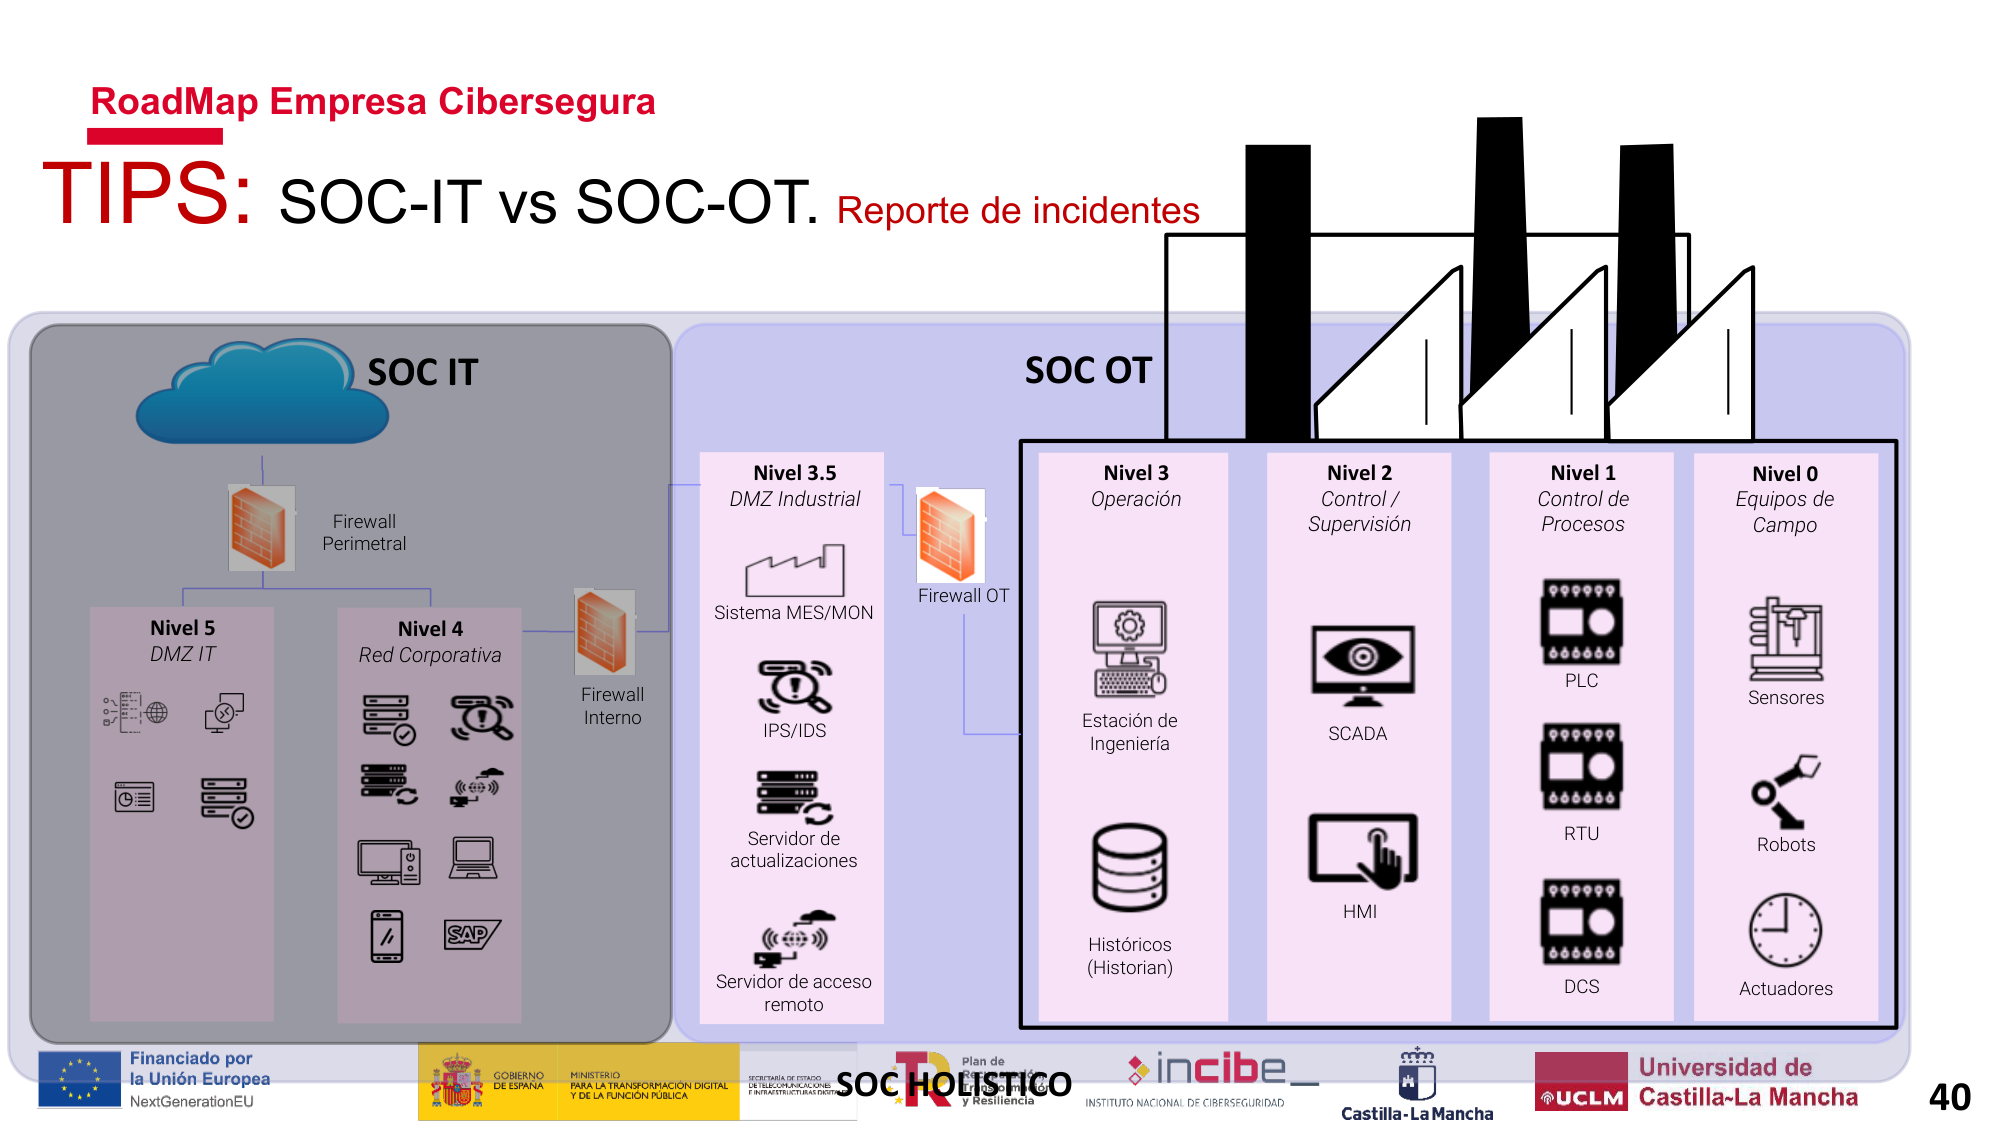
\includegraphics[trim=0 72 0 0,clip,width=\paperwidth,height=\paperheight,keepaspectratio]{img/sl093.png}
\end{frame}

\begin{frame}[allowframebreaks]{El proceso de la seguridad}
\small
  \begin{itemize}
  \item Idea para llevarse:
  \item La seguridad total no existe: es un PROCESO continuo de resiliencia (proteger, detectar, responder y recuperar), alineado con la normativa --- en cualquier organización, industrial o tecnológica.
  \end{itemize}
\end{frame}

\section{Tipos de auditorías}

\begin{frame}{Tipos de auditorías}
\small
  \begin{itemize}
  \item Auditorías Normativas:
    \begin{itemize}
    \item Evaluar el cumplimiento de determinados estándares o requisitos legales.
    \end{itemize}
  \item Auditorías Técnicas:
    \begin{itemize}
    \item Comprobar el estado de nuestra tecnología, compañía o servicio respecto a distintas situaciones.
    \end{itemize}
  \end{itemize}
\vfill
\begin{center}
\includegraphics[width=0.62\textwidth,height=0.55\textheight,keepaspectratio]{img/sl096.jpg}
\end{center}
\end{frame}

\begin{frame}{Tipos de auditorías}
\footnotesize
Cumplimiento normativo
\begin{columns}[c]
\begin{column}{0.74\textwidth}
  \begin{itemize}
  \item RGPD / LOPD
  \item Esquema Nacional de Seguridad
  \item PCI-DSS
  \item ISO 27001
  \item Análisis de riesgos
  \item Especifica los requisitos necesarios para establecer, implantar, mantener y mejorar un sistema de gestión de la seguridad de la información (SGSI)
  \item ISO 22301: Continuidad de negocio
  \item Plan de continuidad y Planes de contingencia
  \item Certificación : proporciona todos los requisitos necesarios para diseñar, implantar, mejorar y certificar un Sistema de Gestión de Continuidad del Negocio.
  \end{itemize}
\end{column}
\begin{column}{0.24\textwidth}
\begin{center}
\includegraphics[width=\textwidth,height=0.5\textheight,keepaspectratio]{img/sl097.jpg}
\end{center}
\end{column}
\end{columns}
\end{frame}

\begin{frame}{Tipos de auditorías}
\begin{center}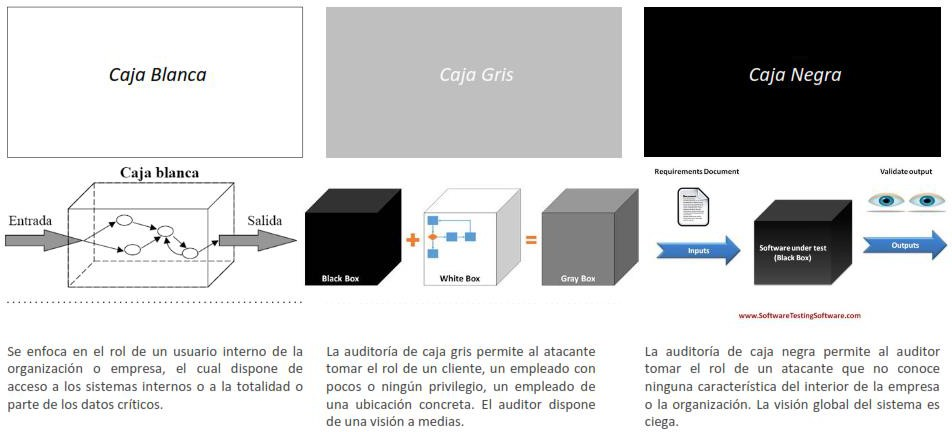
\includegraphics[width=\textwidth,height=0.92\textheight,keepaspectratio]{img/sl098.jpg}
\end{center}
\end{frame}

\begin{frame}{Tipos de auditorías}
\small
Auditorías Técnicas
\begin{columns}[c]
\begin{column}{0.56\textwidth}
  \begin{itemize}
  \item Pentesting
  \item Auditoría Perimetral de red y sistemas
  \item Auditoría Interna de red y sistemas
  \item Análisis de APTs (Malware) / Threat Modelling
  \item Análisis Forense
  \item judicial o no
  \end{itemize}
\end{column}
\begin{column}{0.42\textwidth}
\begin{center}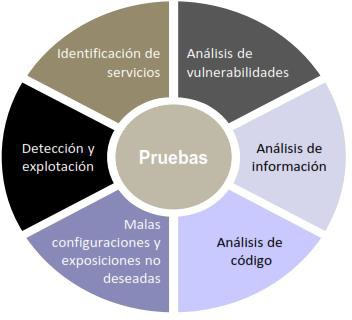
\includegraphics[width=\textwidth,height=0.72\textheight,keepaspectratio]{img/sl099.jpg}
\end{center}
\end{column}
\end{columns}
\end{frame}

\begin{frame}{Tipos de auditorías}
\small
Estándares y modelos. Ejemplo: OWASP
  \begin{itemize}
  \item Organización sin fines de lucro, que proporciona recursos gratuitos para la comunidad.
  \item OWASP recomienda enfocar la seguridad en aplicaciones informáticas considerando las dimensiones de persona, proceso y tecnología.
  \end{itemize}
\vfill
\begin{center}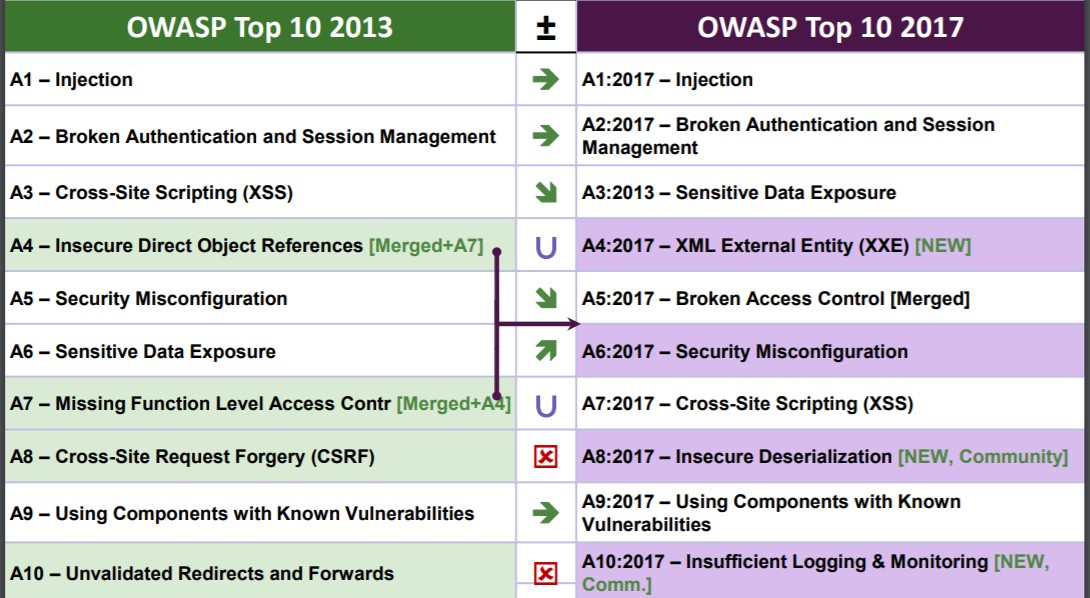
\includegraphics[width=0.7\textwidth,height=0.6\textheight,keepaspectratio]{img/sl100.jpg}
\end{center}
\end{frame}

\begin{frame}[allowframebreaks]{Tipos de auditorías}
\small
  \begin{itemize}
  \item \href{http://seguridad-informacion.blogspot.com/2020/07/red-team-blue-team-y-purple-team-cuales.html}{Lectura} y \href{https://www.youtube.com/watch?v=PXWZZXhz00A}{Lectura}
  \end{itemize}
\begin{center}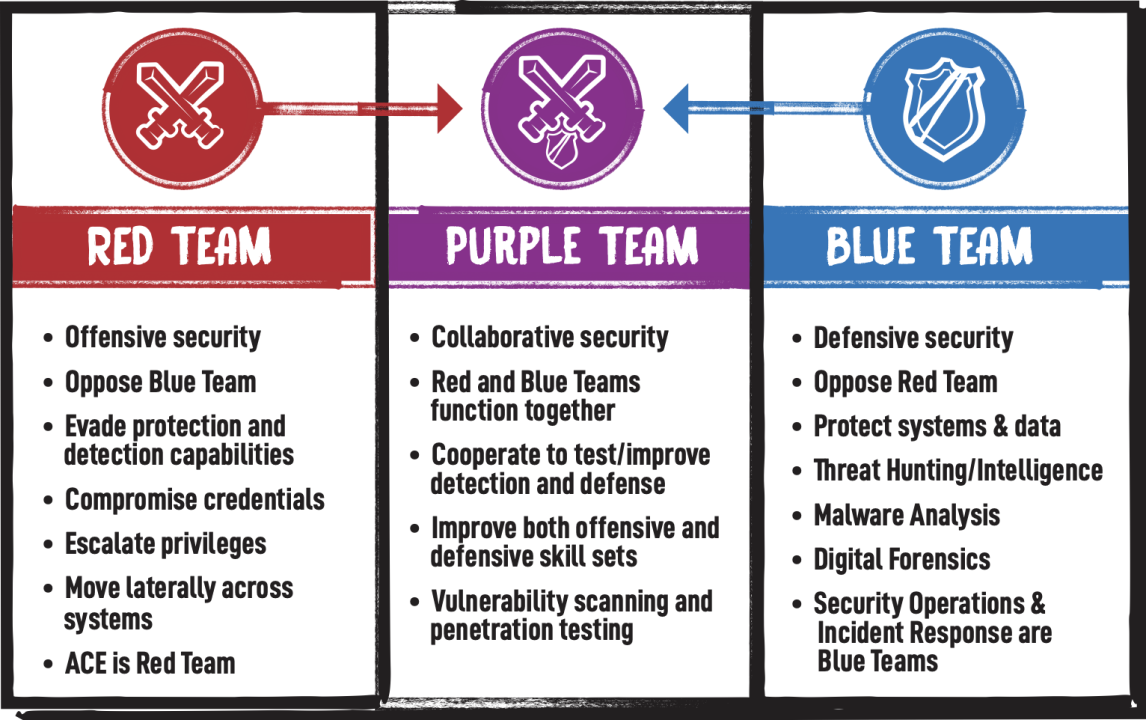
\includegraphics[width=0.72\textwidth,height=0.58\textheight,keepaspectratio]{img/sl101.png}
\end{center}
\end{frame}

\section{Conclusiones}

\begin{frame}[allowframebreaks]{Conclusiones}
\small
  \begin{itemize}
  \item La seguridad de la información se sostiene sobre la triada CIA: Confidencialidad, Integridad y Disponibilidad.
  \item Las vulnerabilidades se identifican y miden de forma estándar (CVE, CVSS) y su gestión es continua, incluidos los 0-day.
  \item Las amenazas van del usuario descuidado y el cracker hasta las APT y los Estados; MITRE ATT\&CK las sistematiza.
  \item El marco legal y normativo (RGPD, ENS, ISO 27001, NIS2) obliga y guía la protección.
  \item Proteger es un proceso de resiliencia: prevenir, detectar, responder y recuperar, apoyado en auditorías y en un SOC.
  \item La seguridad total no existe: es un camino, no un destino.
  \end{itemize}
\end{frame}

\begin{frame}[plain]
  \begin{center}
    {\Huge\bfseries\color{uznavy} ¡Gracias!}\\[1em]
    {\large Seguridad en Sistemas Informáticos --- Tema 1.2}
  \end{center}
\end{frame}

\end{document}